
%% bare_conf.tex
%% V1.3
%% 2007/01/11
%% by Michael Shell
%% See:
%% http://www.michaelshell.org/
%% for current contact information.
%%
%% This is a skeleton file demonstrating the use of IEEEtran.cls
%% (requires IEEEtran.cls version 1.7 or later) with an IEEE conference paper.
%%
%% Support sites:
%% http://www.michaelshell.org/tex/ieeetran/
%% http://www.ctan.org/tex-archive/macros/latex/contrib/IEEEtran/
%% and
%% http://www.ieee.org/

%%*************************************************************************
%% Legal Notice:
%% This code is offered as-is without any warranty either expressed or
%% implied; without even the implied warranty of MERCHANTABILITY or
%% FITNESS FOR A PARTICULAR PURPOSE! 
%% User assumes all risk.
%% In no event shall IEEE or any contributor to this code be liable for
%% any damages or losses, including, but not limited to, incidental,
%% consequential, or any other damages, resulting from the use or misuse
%% of any information contained here.
%%
%% All comments are the opinions of their respective authors and are not
%% necessarily endorsed by the IEEE.
%%
%% This work is distributed under the LaTeX Project Public License (LPPL)
%% ( http://www.latex-project.org/ ) version 1.3, and may be freely used,
%% distributed and modified. A copy of the LPPL, version 1.3, is included
%% in the base LaTeX documentation of all distributions of LaTeX released
%% 2003/12/01 or later.
%% Retain all contribution notices and credits.
%% ** Modified files should be clearly indicated as such, including  **
%% ** renaming them and changing author support contact information. **
%%
%% File list of work: IEEEtran.cls, IEEEtran_HOWTO.pdf, bare_adv.tex,
%%                    bare_conf.tex, bare_jrnl.tex, bare_jrnl_compsoc.tex
%%*************************************************************************

% *** Authors should verify (and, if needed, correct) their LaTeX system  ***
% *** with the testflow diagnostic prior to trusting their LaTeX platform ***
% *** with production work. IEEE's font choices can trigger bugs that do  ***
% *** not appear when using other class files.                            ***
% The testflow support page is at:
% http://www.michaelshell.org/tex/testflow/



% Note that the a4paper option is mainly intended so that authors in
% countries using A4 can easily print to A4 and see how their papers will
% look in print - the typesetting of the document will not typically be
% affected with changes in paper size (but the bottom and side margins will).
% Use the testflow package mentioned above to verify correct handling of
% both paper sizes by the user's LaTeX system.
%
% Also note that the "draftcls" or "draftclsnofoot", not "draft", option
% should be used if it is desired that the figures are to be displayed in
% draft mode.
%
\documentclass[conference]{IEEEtran}
% Add the compsoc option for Computer Society conferences.
%
% If IEEEtran.cls has not been installed into the LaTeX system files,
% manually specify the path to it like:
% \documentclass[conference]{../sty/IEEEtran}





% Some very useful LaTeX packages include:
% (uncomment the ones you want to load)


% *** MISC UTILITY PACKAGES ***
%
%\usepackage{ifpdf}
% Heiko Oberdiek's ifpdf.sty is very useful if you need conditional
% compilation based on whether the output is pdf or dvi.
% usage:
% \ifpdf
%   % pdf code
% \else
%   % dvi code
% \fi
% The latest version of ifpdf.sty can be obtained from:
% http://www.ctan.org/tex-archive/macros/latex/contrib/oberdiek/
% Also, note that IEEEtran.cls V1.7 and later provides a builtin
% \ifCLASSINFOpdf conditional that works the same way.
% When switching from latex to pdflatex and vice-versa, the compiler may
% have to be run twice to clear warning/error messages.






% *** CITATION PACKAGES ***
%
\usepackage{cite}
% cite.sty was written by Donald Arseneau
% V1.6 and later of IEEEtran pre-defines the format of the cite.sty package
% \cite{} output to follow that of IEEE. Loading the cite package will
% result in citation numbers being automatically sorted and properly
% "compressed/ranged". e.g., [1], [9], [2], [7], [5], [6] without using
% cite.sty will become [1], [2], [5]--[7], [9] using cite.sty. cite.sty's
% \cite will automatically add leading space, if needed. Use cite.sty's
% noadjust option (cite.sty V3.8 and later) if you want to turn this off.
% cite.sty is already installed on most LaTeX systems. Be sure and use
% version 4.0 (2003-05-27) and later if using hyperref.sty. cite.sty does
% not currently provide for hyperlinked citations.
% The latest version can be obtained at:
% http://www.ctan.org/tex-archive/macros/latex/contrib/cite/
% The documentation is contained in the cite.sty file itself.






% *** GRAPHICS RELATED PACKAGES ***
%
\ifCLASSINFOpdf
   \usepackage[pdftex]{graphicx}
  % declare the path(s) where your graphic files are
   \graphicspath{{../pdf/}{../jpeg/}}
  % and their extensions so you won't have to specify these with
  % every instance of \includegraphics
   \DeclareGraphicsExtensions{.pdf,.jpeg,.png}
\else
  % or other class option (dvipsone, dvipdf, if not using dvips). graphicx
  % will default to the driver specified in the system graphics.cfg if no
  % driver is specified.
  % \usepackage[dvips]{graphicx}
  % declare the path(s) where your graphic files are
  % \graphicspath{{../eps/}}
  % and their extensions so you won't have to specify these with
  % every instance of \includegraphics
  % \DeclareGraphicsExtensions{.eps}
\fi
% graphicx was written by David Carlisle and Sebastian Rahtz. It is
% required if you want graphics, photos, etc. graphicx.sty is already
% installed on most LaTeX systems. The latest version and documentation can
% be obtained at: 
% http://www.ctan.org/tex-archive/macros/latex/required/graphics/
% Another good source of documentation is "Using Imported Graphics in
% LaTeX2e" by Keith Reckdahl which can be found as epslatex.ps or
% epslatex.pdf at: http://www.ctan.org/tex-archive/info/
%
% latex, and pdflatex in dvi mode, support graphics in encapsulated
% postscript (.eps) format. pdflatex in pdf mode supports graphics
% in .pdf, .jpeg, .png and .mps (metapost) formats. Users should ensure
% that all non-photo figures use a vector format (.eps, .pdf, .mps) and
% not a bitmapped formats (.jpeg, .png). IEEE frowns on bitmapped formats
% which can result in "jaggedy"/blurry rendering of lines and letters as
% well as large increases in file sizes.
%
% You can find documentation about the pdfTeX application at:
% http://www.tug.org/applications/pdftex





% *** MATH PACKAGES ***
%
\usepackage[cmex10]{amsmath}
\usepackage{amssymb}
% A popular package from the American Mathematical Society that provides
% many useful and powerful commands for dealing with mathematics. If using
% it, be sure to load this package with the cmex10 option to ensure that
% only type 1 fonts will utilized at all point sizes. Without this option,
% it is possible that some math symbols, particularly those within
% footnotes, will be rendered in bitmap form which will result in a
% document that can not be IEEE Xplore compliant!
%
% Also, note that the amsmath package sets \interdisplaylinepenalty to 10000
% thus preventing page breaks from occurring within multiline equations. Use:
\interdisplaylinepenalty=2500
% after loading amsmath to restore such page breaks as IEEEtran.cls normally
% does. amsmath.sty is already installed on most LaTeX systems. The latest
% version and documentation can be obtained at:
% http://www.ctan.org/tex-archive/macros/latex/required/amslatex/math/





% *** SPECIALIZED LIST PACKAGES ***
%
\usepackage{algorithm}
\usepackage{algorithmic}
\renewcommand{\algorithmicrequire}{\textbf{Input:}} 
\renewcommand{\algorithmicensure}{\textbf{Output:}}
% algorithmic.sty was written by Peter Williams and Rogerio Brito.
% This package provides an algorithmic environment fo describing algorithms.
% You can use the algorithmic environment in-text or within a figure
% environment to provide for a floating algorithm. Do NOT use the algorithm
% floating environment provided by algorithm.sty (by the same authors) or
% algorithm2e.sty (by Christophe Fiorio) as IEEE does not use dedicated
% algorithm float types and packages that provide these will not provide
% correct IEEE style captions. The latest version and documentation of
% algorithmic.sty can be obtained at:
% http://www.ctan.org/tex-archive/macros/latex/contrib/algorithms/
% There is also a support site at:
% http://algorithms.berlios.de/index.html
% Also of interest may be the (relatively newer and more customizable)
% algorithmicx.sty package by Szasz Janos:
% http://www.ctan.org/tex-archive/macros/latex/contrib/algorithmicx/




% *** ALIGNMENT PACKAGES ***
%
\usepackage{array}
% Frank Mittelbach's and David Carlisle's array.sty patches and improves
% the standard LaTeX2e array and tabular environments to provide better
% appearance and additional user controls. As the default LaTeX2e table
% generation code is lacking to the point of almost being broken with
% respect to the quality of the end results, all users are strongly
% advised to use an enhanced (at the very least that provided by array.sty)
% set of table tools. array.sty is already installed on most systems. The
% latest version and documentation can be obtained at:
% http://www.ctan.org/tex-archive/macros/latex/required/tools/


\usepackage{mdwmath}
\usepackage{mdwtab}
% Also highly recommended is Mark Wooding's extremely powerful MDW tools,
% especially mdwmath.sty and mdwtab.sty which are used to format equations
% and tables, respectively. The MDWtools set is already installed on most
% LaTeX systems. The lastest version and documentation is available at:
% http://www.ctan.org/tex-archive/macros/latex/contrib/mdwtools/


% IEEEtran contains the IEEEeqnarray family of commands that can be used to
% generate multiline equations as well as matrices, tables, etc., of high
% quality.


\usepackage{eqparbox}
% Also of notable interest is Scott Pakin's eqparbox package for creating
% (automatically sized) equal width boxes - aka "natural width parboxes".
% Available at:
% http://www.ctan.org/tex-archive/macros/latex/contrib/eqparbox/





% *** SUBFIGURE PACKAGES ***
\usepackage[tight,footnotesize]{subfigure}
% subfigure.sty was written by Steven Douglas Cochran. This package makes it
% easy to put subfigures in your figures. e.g., "Figure 1a and 1b". For IEEE
% work, it is a good idea to load it with the tight package option to reduce
% the amount of white space around the subfigures. subfigure.sty is already
% installed on most LaTeX systems. The latest version and documentation can
% be obtained at:
% http://www.ctan.org/tex-archive/obsolete/macros/latex/contrib/subfigure/
% subfigure.sty has been superceeded by subfig.sty.



%\usepackage[caption=false]{caption}
%\usepackage[font=footnotesize]{subfig}
% subfig.sty, also written by Steven Douglas Cochran, is the modern
% replacement for subfigure.sty. However, subfig.sty requires and
% automatically loads Axel Sommerfeldt's caption.sty which will override
% IEEEtran.cls handling of captions and this will result in nonIEEE style
% figure/table captions. To prevent this problem, be sure and preload
% caption.sty with its "caption=false" package option. This is will preserve
% IEEEtran.cls handing of captions. Version 1.3 (2005/06/28) and later 
% (recommended due to many improvements over 1.2) of subfig.sty supports
% the caption=false option directly:
%\usepackage[caption=false,font=footnotesize]{subfig}
%
% The latest version and documentation can be obtained at:
% http://www.ctan.org/tex-archive/macros/latex/contrib/subfig/
% The latest version and documentation of caption.sty can be obtained at:
% http://www.ctan.org/tex-archive/macros/latex/contrib/caption/




% *** FLOAT PACKAGES ***
%
%\usepackage{fixltx2e}
% fixltx2e, the successor to the earlier fix2col.sty, was written by
% Frank Mittelbach and David Carlisle. This package corrects a few problems
% in the LaTeX2e kernel, the most notable of which is that in current
% LaTeX2e releases, the ordering of single and double column floats is not
% guaranteed to be preserved. Thus, an unpatched LaTeX2e can allow a
% single column figure to be placed prior to an earlier double column
% figure. The latest version and documentation can be found at:
% http://www.ctan.org/tex-archive/macros/latex/base/



%\usepackage{stfloats}
% stfloats.sty was written by Sigitas Tolusis. This package gives LaTeX2e
% the ability to do double column floats at the bottom of the page as well
% as the top. (e.g., "\begin{figure*}[!b]" is not normally possible in
% LaTeX2e). It also provides a command:
%\fnbelowfloat
% to enable the placement of footnotes below bottom floats (the standard
% LaTeX2e kernel puts them above bottom floats). This is an invasive package
% which rewrites many portions of the LaTeX2e float routines. It may not work
% with other packages that modify the LaTeX2e float routines. The latest
% version and documentation can be obtained at:
% http://www.ctan.org/tex-archive/macros/latex/contrib/sttools/
% Documentation is contained in the stfloats.sty comments as well as in the
% presfull.pdf file. Do not use the stfloats baselinefloat ability as IEEE
% does not allow \baselineskip to stretch. Authors submitting work to the
% IEEE should note that IEEE rarely uses double column equations and
% that authors should try to avoid such use. Do not be tempted to use the
% cuted.sty or midfloat.sty packages (also by Sigitas Tolusis) as IEEE does
% not format its papers in such ways.





% *** PDF, URL AND HYPERLINK PACKAGES ***
%
%\usepackage{url}
% url.sty was written by Donald Arseneau. It provides better support for
% handling and breaking URLs. url.sty is already installed on most LaTeX
% systems. The latest version can be obtained at:
% http://www.ctan.org/tex-archive/macros/latex/contrib/misc/
% Read the url.sty source comments for usage information. Basically,
% \url{my_url_here}.





% *** Do not adjust lengths that control margins, column widths, etc. ***
% *** Do not use packages that alter fonts (such as pslatex).         ***
% There should be no need to do such things with IEEEtran.cls V1.6 and later.
% (Unless specifically asked to do so by the journal or conference you plan
% to submit to, of course. )


% correct bad hyphenation here
\hyphenation{op-tical net-works semi-conduc-tor}


\begin{document}
%
% paper title
% can use linebreaks \\ within to get better formatting as desired
\title{GTS: An In-memory GPU-accelerated Trajectory Storage System For Basic Spatial Queries}


% author names and affiliations
% use a multiple column layout for up to three different
% affiliations
\author{\IEEEauthorblockN{Zhang Bowen}
\IEEEauthorblockA{Department of Computer Science and Engeneering\\
Shanghai Jiao Tong University\\
Shanghai, China 200240\\
Email: zbw0046@sjtu.edu.cn}}
%\and
%\IEEEauthorblockN{Homer Simpson}
%\IEEEauthorblockA{Twentieth Century Fox\\
%Springfield, USA\\
%Email: homer@thesimpsons.com}
%\and
%\IEEEauthorblockN{James Kirk\\ and Montgomery Scott}
%\IEEEauthorblockA{Starfleet Academy\\
%San Francisco, California 96678-2391\\
%Telephone: (800) 555--1212\\
%Fax: (888) 555--1212}}

% conference papers do not typically use \thanks and this command
% is locked out in conference mode. If really needed, such as for
% the acknowledgment of grants, issue a \IEEEoverridecommandlockouts
% after \documentclass

% for over three affiliations, or if they all won't fit within the width
% of the page, use this alternative format:
% 
%\author{\IEEEauthorblockN{Michael Shell\IEEEauthorrefmark{1},
%Homer Simpson\IEEEauthorrefmark{2},
%James Kirk\IEEEauthorrefmark{3}, 
%Montgomery Scott\IEEEauthorrefmark{3} and
%Eldon Tyrell\IEEEauthorrefmark{4}}
%\IEEEauthorblockA{\IEEEauthorrefmark{1}School of Electrical and Computer Engineering\\
%Georgia Institute of Technology,
%Atlanta, Georgia 30332--0250\\ Email: see http://www.michaelshell.org/contact.html}
%\IEEEauthorblockA{\IEEEauthorrefmark{2}Twentieth Century Fox, Springfield, USA\\
%Email: homer@thesimpsons.com}
%\IEEEauthorblockA{\IEEEauthorrefmark{3}Starfleet Academy, San Francisco, California 96678-2391\\
%Telephone: (800) 555--1212, Fax: (888) 555--1212}
%\IEEEauthorblockA{\IEEEauthorrefmark{4}Tyrell Inc., 123 Replicant Street, Los Angeles, California 90210--4321}}




% use for special paper notices
%\IEEEspecialpapernotice{(Invited Paper)}




% make the title area
\maketitle


\begin{abstract}
%\boldmath
As the development of smart devices equipped with GPS, here comes a large amount of trajectory data, implying many useful information about our daily life. This call for a trajectory storage system able to handle mass of various kinds of queries efficiently. GPU, which has been widely equipped on computers, can accelerate queries by handling them in parallel. However, existing GPU-accelerated trajectory storage systems are optimized for specific kind of query, unable to support wide range of applications. To solve this problem, we propose a storage system optimized for the features of GPU, supporting multiple kinds of queries. We exploit the potential opportunities of PR-quadtree in adapting to different strategies for pruning, designing an adaptive storage component. To make full use of the parallel power of GPU, we develop a query engine optimized with load-balancing, coalesce memory accessing and less data transferring. We evaluate our system on trajectory dataset of cars in Shanghai, which shows our system able to conduct three basic kinds of queries efficiently. Moreover, our system speed up about 10x for EDR measured top-k similarity query than implementing on CPU, demonstrating that GPU can be used to accelerate queries on large-scale trajectory data.


\end{abstract}
% IEEEtran.cls defaults to using nonbold math in the Abstract.
% This preserves the distinction between vectors and scalars. However,
% if the conference you are submitting to favors bold math in the abstract,
% then you can use LaTeX's standard command \boldmath at the very start
% of the abstract to achieve this. Many IEEE journals/conferences frown on
% math in the abstract anyway.

% no keywords




% For peer review papers, you can put extra information on the cover
% page as needed:
% \ifCLASSOPTIONpeerreview
% \begin{center} \bfseries EDICS Category: 3-BBND \end{center}
% \fi
%
% For peerreview papers, this IEEEtran command inserts a page break and
% creates the second title. It will be ignored for other modes.
\IEEEpeerreviewmaketitle



\section{Introduction}
% no \IEEEPARstart
	\textbf{background}
	
	As the number of mobile location devices (like smartphones, cars, public bicycles, etc.) grows, increasing amount of spatial-temporal sequential data, i.e. trajectory data is collected from the every corner of the world. For example, 80GB trajectory data are generated during July 1, 2013 and April 30, 2014 just from private cars in Shanghai, which contains more than 247,494,133 sample points. There are many interesting and valuable information in these data to be exploited, such as route planing[...], traffic prediction[...], travel time prediction\cite{DBLP:conf/gis/LeeSCC12} etc.. Thousands of queries are produced everyday in these applications. They call for a solution of efficient trajectory storage and retrieval. Recent years various kinds of spatial indexes and in-memory storage are proposed to increase throughput and decrease latency. Meanwhile, having witnessed the growing application of GPU in large-scale data processing, it is a popular choice that use it to answer mass of queries in parallel\cite{7498315}[...]. As a many-core architecture processor, GPU can achieve high throughtput by handling thousands of threads at a time.
	
	\textbf{problem description}
	
	Although a mass of query algorithm are designed for different purposes recently, they can be concluded in two main types: range-based query and trajectory-based query, which can be represented by two basic type of spatial queries: range query and top-k trajectory similarity query respectively.\cite{DBLP:journals/tist/Zheng15} This two kinds of query are both indispensable for many kinds of trajectory applications. For example, they are both invoked in the process of travel time prediction\cite{DBLP:conf/gis/LeeSCC12}. In this situation, query delay is significantly important for user's experience. So, it is valuable to develope a trajectory storage system which can make use of GPU to efficiently execute those different kinds of queries in a short response time. However, existing trajectory storage systems are almost optimized for specific kind of query on CPU, causing that applications invoking different kinds of query lose efficiency when running on them. Also, the index designed for CPU cannot be easily migrated to GPU because of the significantly different architecture. It is not wise to trivially add an additional query module to support the queries not included in their original optimization consideration because of the low pruning performance caused by mismatching index not optimized for this kind of query. 
	% we lack a trajectory database which can handle all three kinds of queries. 
	
		(picture of two kinds of query)
	%交代随着智能定位设备数量的增长,轨迹数据规模越来越大,以及设计出了内存数据库和GPU加速的查询……并罗列数据说明
	
	
\textbf{challenge of solving problem}


	% 要详细展开写嘛?
	
	However, to implement this idea, there are some main challenges in both storage designing and query algorithm designing.
	(i) Firstly, it is difficult to design index optimized for both two types of query at the same time. In existing work, people use location-based index which is metric to handle range query, for example, kd-tree. This type of queries allows for the usage of triangle inequality because of its metric property. However, local time shifting based trajectory similarity query, such as \cite{DBLP:conf/sigmod/ChenOO05}, calls for pruning methods which is based on inequation derived from the properties of similarity measurements, which is usually not metric.
	To solve this problem, it is intuitive to set two database for different kind of query respectively. Unfortunately, this will cause unneccessary space comsumption because of duplicate data are stored, which is harmful for memory efficiency. Considering that less space consumption means a mass of benefits for trajectory data mining, such as more trajectories can be persisted in main memory as training set to improve accuracy, it's neccessary to find a space-saving solution.
	% 连续存储不是一个问题,因为SharkDB也可以连续存储,根本问题在于是否metric
	%kNN query and range query need location-based storage such as splitting whole trajectory into sub-trajectories. However, it is integral to read whole trajectory firstly for similarity query, which location-based storage can't support efficiently. One solution is use two independent indices for this three kinds of query, but noting that improving memory efficiency has many benefits for in-memory database(cited by Huanchen Zhang), it's too expensive for in-memory system because of high space consumption. 
	
	(ii) Secondly, there is no proper task division strategy used to improve query performance for some queries oriented to data-level parallelization device such as GPU. We will take EDR, a local time shifting based similarity measurements, as an example. For some simpler similarity measurements such as Hasdoff distance\cite{DBLP:conf/bigdataconf/LealGZY15}, parallelization of similarity query algorithm is easily implemented by dividing whole trajectory into segments first and then assigning each segment to a thread to handle.\cite{DBLP:conf/bigdataconf/LealGZY15} However, different from this, calculation of EDR is correlated with all points of trajectory, which means a global optimal alignment, disallowing the division of the trajectory in the process of computation. 
	
	(iii) Thirdly, because of the architecture limits of GPU, there are many issues should be concerned when designing data layout method and index\cite{7498315}. For example, memory accessing pattern is a main concern when designing algorithm oriented to GPU, which require us to coalesce the locations of data requests from a warp of threads to a continuous space in global memory of GPU to avoid the high latency when thousands of cores access memory. Sometimes an efficient index working on CPU may disallow this requirement, so it should be specially re-designed if we want to make it work efficiently on GPU.
	
	% in traditional tree-based trajectory index such as R-tree, pruning is implemented by search every node recursively. However, recursive operation is not efficiently support by GPU because of different architecture from CPU. This claims that we should 
	
	(I'm finding more challenge...)
	%	ii.
	%	
	%	iii.There are lots of barriers when using GPU to handle queries parallel such as low speed of PCI-Express between host memory and GPU. \textbf{It's impratical to store all data in GPU memory which is so small, so this gap between host memory to GPU can be a bottleneck of system.}
	%	
	%	iv.It is easy to develop index and data structure aiming at one given kind of query, but difficult when aiming at three kinds of query. Storing multiple indices for each kind of query may solve this problem but make it consume a large portion of main memory.
	
	
\textbf{existing work about this problem}
	% (先把问题全部列出来,看哪些能解决再最后写上)
	
	i.SharkDB propose a column-based data structure to store trajectory data leverageing the time-aggregation of queries. But it can't support trajectory-based query, such as trajectory similarity query because column-based storage makes it hard to access the whole trajectory sequence fastly, which is an important step in similarity query. Besides, the parallel query algorithm that SharkDB develope is only for thread pool, which can't easily migrate to GPU.
	
	ii.TKSimGPU propose a query algorithm that implemented on GPU which is designed for trajectory similarity query. However, the similarity measurement which TKSimGPU use is outdated, because it doesn't take local time shifting into concern, which has been proved a significant issue for similarity measurement of trajectory(cited by DTW,EDR,...). Moreover, range query is not supported efficiently by TKSimGPU because of non-adaptive grid.
	
\textbf{my idea}
	
	%i.
	In this work, to solve this problem, we design and implement the GTS (\underline{G}PU-accelerated \underline{T}rajectory \underline{S}torage) system, which can handle both range query and local time shifting based top-k similarity query on historical trajectory data. Recent years many similarity measurements based on local time shifting are proposed and be verificated outperforming traditional Euclidean distance based measurements[][]. So it is important for trajectory storage system to support this kind of query. We design a single storage component supporting pruning on both two kinds of query with no duplicated data, to save memory space. Moreover, our design is friendly with GPU, which means we can make use of parallel power of it to accelerate query engine. It is worth mentioning that we are the first one to design top-k similarity query algorithm for GPU supporting local time shifting. 
	
	%For different kinds of query, we try to develope uniform index through analysing the features of reading trajectory samples under corresponding query. For example, it is worth to note that the most state-of-the-art similarity measurement between different trajectories,such as DTW,LCSS and EDR, are based on dynamic programming. This observation inspires us to use data structure which is friendly when accessing the whole trajectory. 
	

	
\textbf{main solutions}

	i. To address the challenge (i), we propose a novel trajectory storage component based on quadtree. We find that data structures used in pruning process of EDR is similar with grid, which has been widely used as index for GPU-accelerated range query. On the basic of this observation, we subtly adopt the characters of Morton encoding and PR-quadtree to design an index supporting pruning both on range query and top-k similarity query.
	%i.
	
	ii. To address the challenge (ii), we design the query algorithm which is load balancing and has the coalesce accessing pattern to avoid the performance loss caused by improper memory accessing pattern. For top-k similarity search, we leverage the potential independence of the procedure to design a scalable task division strategy considering both coarse-grain and fine-grain parallelism to make full use of GPU's parallel power. Otherwise, we design a special placement organization of elements in state matrix in GPU global memory, satisfying the requirement of coalesce accessing.
	%We use partition-based index to handle range query and kNN query, and use bounds which are derived from similarity query's definition to pruning for similarity query. From this design we can save memory space comparing to widely used tree-based index. Inspried from the phenomenon that GPU has been widely equipped on PC and server, we can use GPU to make up the performance loss caused by absence of tree-based index.
%	
%	ii. We use xxx tree to index sample points in each column because this data structure can divide the all points into several parts according to the (location/xxx) features. We can deal with skew data with no performance loss because only a small part(tight) of points are collected as candidate dataset for queries.
%	
%	iii....(some improvement based on GPU parallel programming)
%	
%	iv.For different kinds of query, we try to develope uniform index through analysing the features of reading trajectory samples under corresponding query. For example, it is worth to note that the most state-of-the-art similarity measurement between different trajectories,such as DTW,LCSS and EDR, are based on dynamic programming. By the time, range query and kNN query .This observation inspires us to use data structure which is friendly when accessing the whole trajectory. 
	
\textbf{contributions}

\begin{itemize}
	\item We propose a GPU-accelerated in-memory trajectory storage system which support both range query and local time shifting based top-k similarity query on a single index.
	\item We design an quadtree integrated trajectory storage component, not only works for GPU-accelerated range query but also exploiting GPU's parallel power in accelerating top-k similarity query.
	\item We design a novel solution of accelerating local time shifting based similarity query on our storage component by exploiting GPU's parallel power.
	\item We implement our system on server, evaluate the performance, and prove that our system get 4x speedup for top-k similarity comparing to baseline, and meanwhile, get similar performance on range query comparing to state-of-the-art systems not originally supporting local time shifting based top-k similarity query, with similar memory consumption.
\end{itemize}
	 
\textbf{organization}

	The rest of paper is organized as follows. In Section 2 we review the related work. After that, in section 3 we briefly introduce the architecture of our system. We propose our design of storage component in section 4. Query engine is described in detail in section 5 with three kinds of query algorithm. In section 6, we do an evaluation of our system and results are reported. Section 7 concludes the paper. 



\section{Background}
We first give the preliminaries.
Then we introduce some background knowledge of GPU used in our design.

\subsection{Problem Definition}
	In this section, we propose some basic definition of trajectory and formulation about our problem. We first define some elements of trajectory.
	
	\newtheorem{define}{Definition}
	\begin{define}[sample point]
		A sample point $p=(x,y,time)$ is a three-dimensional data which include spatial information represented by $(x,y)$ and time stamp $time$. For simplicity, we assume that all sample points' coordinates have been transfered to Euclidean plane.
	\end{define}

	\begin{define}[trajectory]
		A trajectory of the object $t=\{p_{1},p_{2},\ldots,p_{n}\}$ is a sequence of sample points, where $n$ is the length of this trajectory. To make the trajectories meaningful, we raise a regulation that the delta of timestamp between two consecutive sample points should be always within 30 minutes. 
	\end{define}

	Given a large set of trajectories $T={t_{1},t_{2},\ldots,t_{|T|}}$, our goal is answering all kinds of queries over them. As we mentioned in Section 1, they can be classified into range query, k-nearest neighbor point query and top-k trajectory similarity query. Here we formulate this three kinds of query.
	
	\begin{define}[query]
		A query $q=(kind,cond,T)$ aims to find a set of trajectories or segments as results $S$ from trajectory dataset $T$ which satisfy query conditions $cond$, where $kind$ is the notation of the kind of the query.
	\end{define}
	
	For range query, the condition usually includes a bounding box $B=[xmin,xmax,ymin,ymax]$ and a time range $[time_{s},time_{e}]$. A trajectory $t$ is said to satisfy range query if there exist at least one sample point $e.p_{1}$ is included in the bounding box and its time stamp is within time range, which can be represented as $\exists p\in t, (xmin \leq p.x \leq xmax) \wedge (ymin \leq p.y \leq ymax) \wedge (time_{s} \leq p.time \leq time_{e})$. 

%	K-nearest neighbor point query retrieves a set of k trajectories $R_{kNN}=\{t_{1},t_{2},\ldots ,t_{k}\}$ which are top-k nearest to given coordinate $(q_{x},q_{y})$. The coordinate and $k$ are contained in query condition. We use the smallest euclidean distance between the coordinate and sample points of trajectory as measurement of nearness.
	
	
	
	Top-k trajectory similarity query retrieves a set of k trajectories $R_{sim}=\{t_{1},t_{2},\ldots ,t_{k}\}$ which are most similar with given trajectory $t_{q}$. There are many metric about trajectory similarity, and it's widely accepted that EDR distance\cite{DBLP:conf/sigmod/ChenOO05} which can handle local time shifting may be a good choice. So we use EDR distance as our similairity metric.
	
	\begin{define}[EDR distance\cite{DBLP:conf/sigmod/ChenOO05}]
		Given two trajectories $t_{1}=\{p_{1},p_{2},\ldots,p_{n1+1}\},t_{2}=\{p_{1},p_{2},\ldots,p_{n2+1}\}$, the EDR distance between them is calculated by:
		\begin{equation}
		EDR(t_{1},t_{2}) = 
		\begin{cases}
		n & \text{if $m=0$} \\
		m & \text{if $n=0$} \\
		\min \{EDR(Rest(t_{1}),\\Rest(t_{2})+subcost),\\EDR(Rest(t_{1}),t_{2})+1,\\EDR(t_{1},Rest(t_{2}))+1\} & \text{otherwise}
		\end{cases}
		\end{equation}
		where $subcost = 0$ if $dist(t_{1}.p_{1},t_{2}.p_{1})\leqslant \varepsilon$ and $subcost = 1$ otherwise, and $Rest(t)=\{t.p_{2},\ldots ,t.p_{n+1}\}$, noting that $\varepsilon$ is a threshold set by users.
	\end{define}
	
%	\begin{figure*}[!t]\centering
%	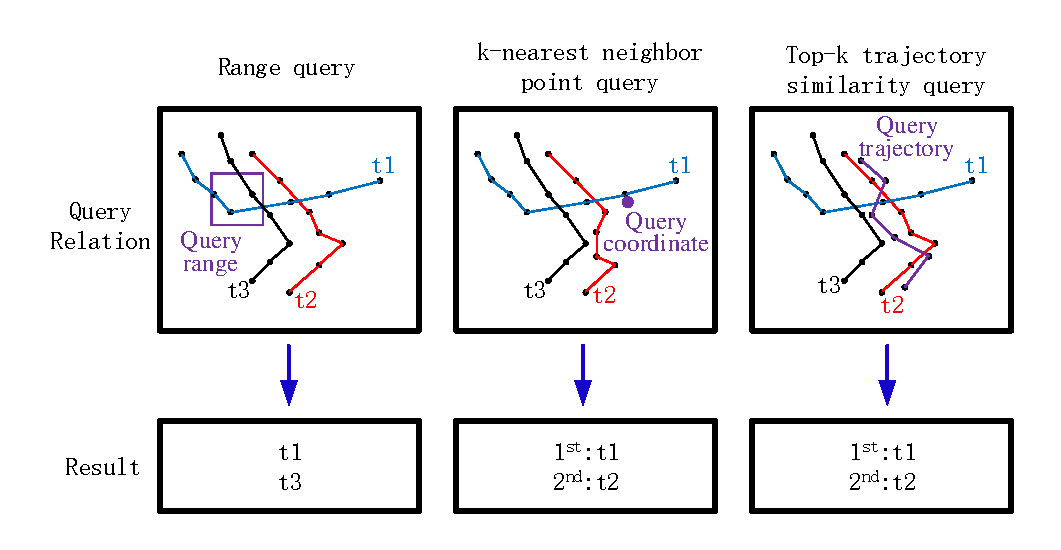
\includegraphics{querykind.pdf}
%	\caption{three kind of query\label{fig:1}}
%	\end{figure*}

\subsection{GPU computing using CUDA[]}
We design GTS based on CUDA proposed by Nvidia, a programming framework for GPU computing. In this part we introduce some background of GPU and basic concept in CUDA. GPU follows Single Intruction Multiple Data (SIMD) parallel model, indicating all of the cores in an Stream Microprocessor (SM) executing the same instruction on different data at the same time. There are tens of SMs in one GPU, each of which has tens of cores, forming a two-level parallel architecture. In CUDA, this architecture is reflected in the division of grid, block and thread. When one program, called kernel, is loaded in CUDA, a grid is generated, including mass of blocks. The block contains a fixed number of threads, which runs on an SM of GPU. Threads in the same block can share a high speed but small volume local memory on SM, and threads in different blocks can use a slower GPU global memory to exchange information. This requires us to divide the task properly into different blocks properly. 

There are three main issues when using GPU. First, accessing pattern is a main issue when accessing global memory. When hundreds of threads in one block read/write data from global memory, if the data each thread needs are nearby, GPU will coalesce hundreds of small accessing request to several big continuous accessing transactions. Because GPU has a high bandwidth but high latency global memory, by this coalescing threads can get needed data in a pretty small number of clock cycles. For example, if thread 1,2,..,32 access the data at offset 33,34,...,64 respectively, 32 data loading requests will be combined to one single transition. So if program access data from global memory, it is optimal when data read/writen by all threads in a block are stored continuously, and ensuring an optimal memory access pattern is significant for making full use of GPU. Second, the load balancing makes sure that all cores of GPU are not idle, leading to a high throughtput. It means we should assign almost equal amount of computation on one thread or one block. Third, there is a tradeoff about the layout of large-scale trajectory data. The capability of GPU global memory is limit, for example, 12GB in most of ultimate level GPU devices. So we may think about store all data in host memory. However, PCI-E interface, the bridge between host memory and GPU, has much lower bandwidth than global memory which is inside GPU. This requires usto reduce data transferring between main memory and GPU as much as possible to avoid the performance loss. Comparing to other parallel computing tools based on multi-core CPU such as MPI, these three issues raise a challenge for GTS to get a high speedup on GPU.

\section{System Architecture}

\subsection{Overview}
Our system includes two parts, storage component and query engine. As the Figure \ref{fig:Archi} shows, raw trajectories are split into sub-trajectories according to quadtree index, with the corresponding sequence of cell stored as cell-based trajectories. After raw trajectories are loaded into storage component, thousands of queries are handled in query engine, with the acceleration of GPGPU, outputing query results. It's worth noting that our system is designed for query-only applications. We then introduce storage component and query engine briefly.

\begin{figure*}[htbp]\centering
	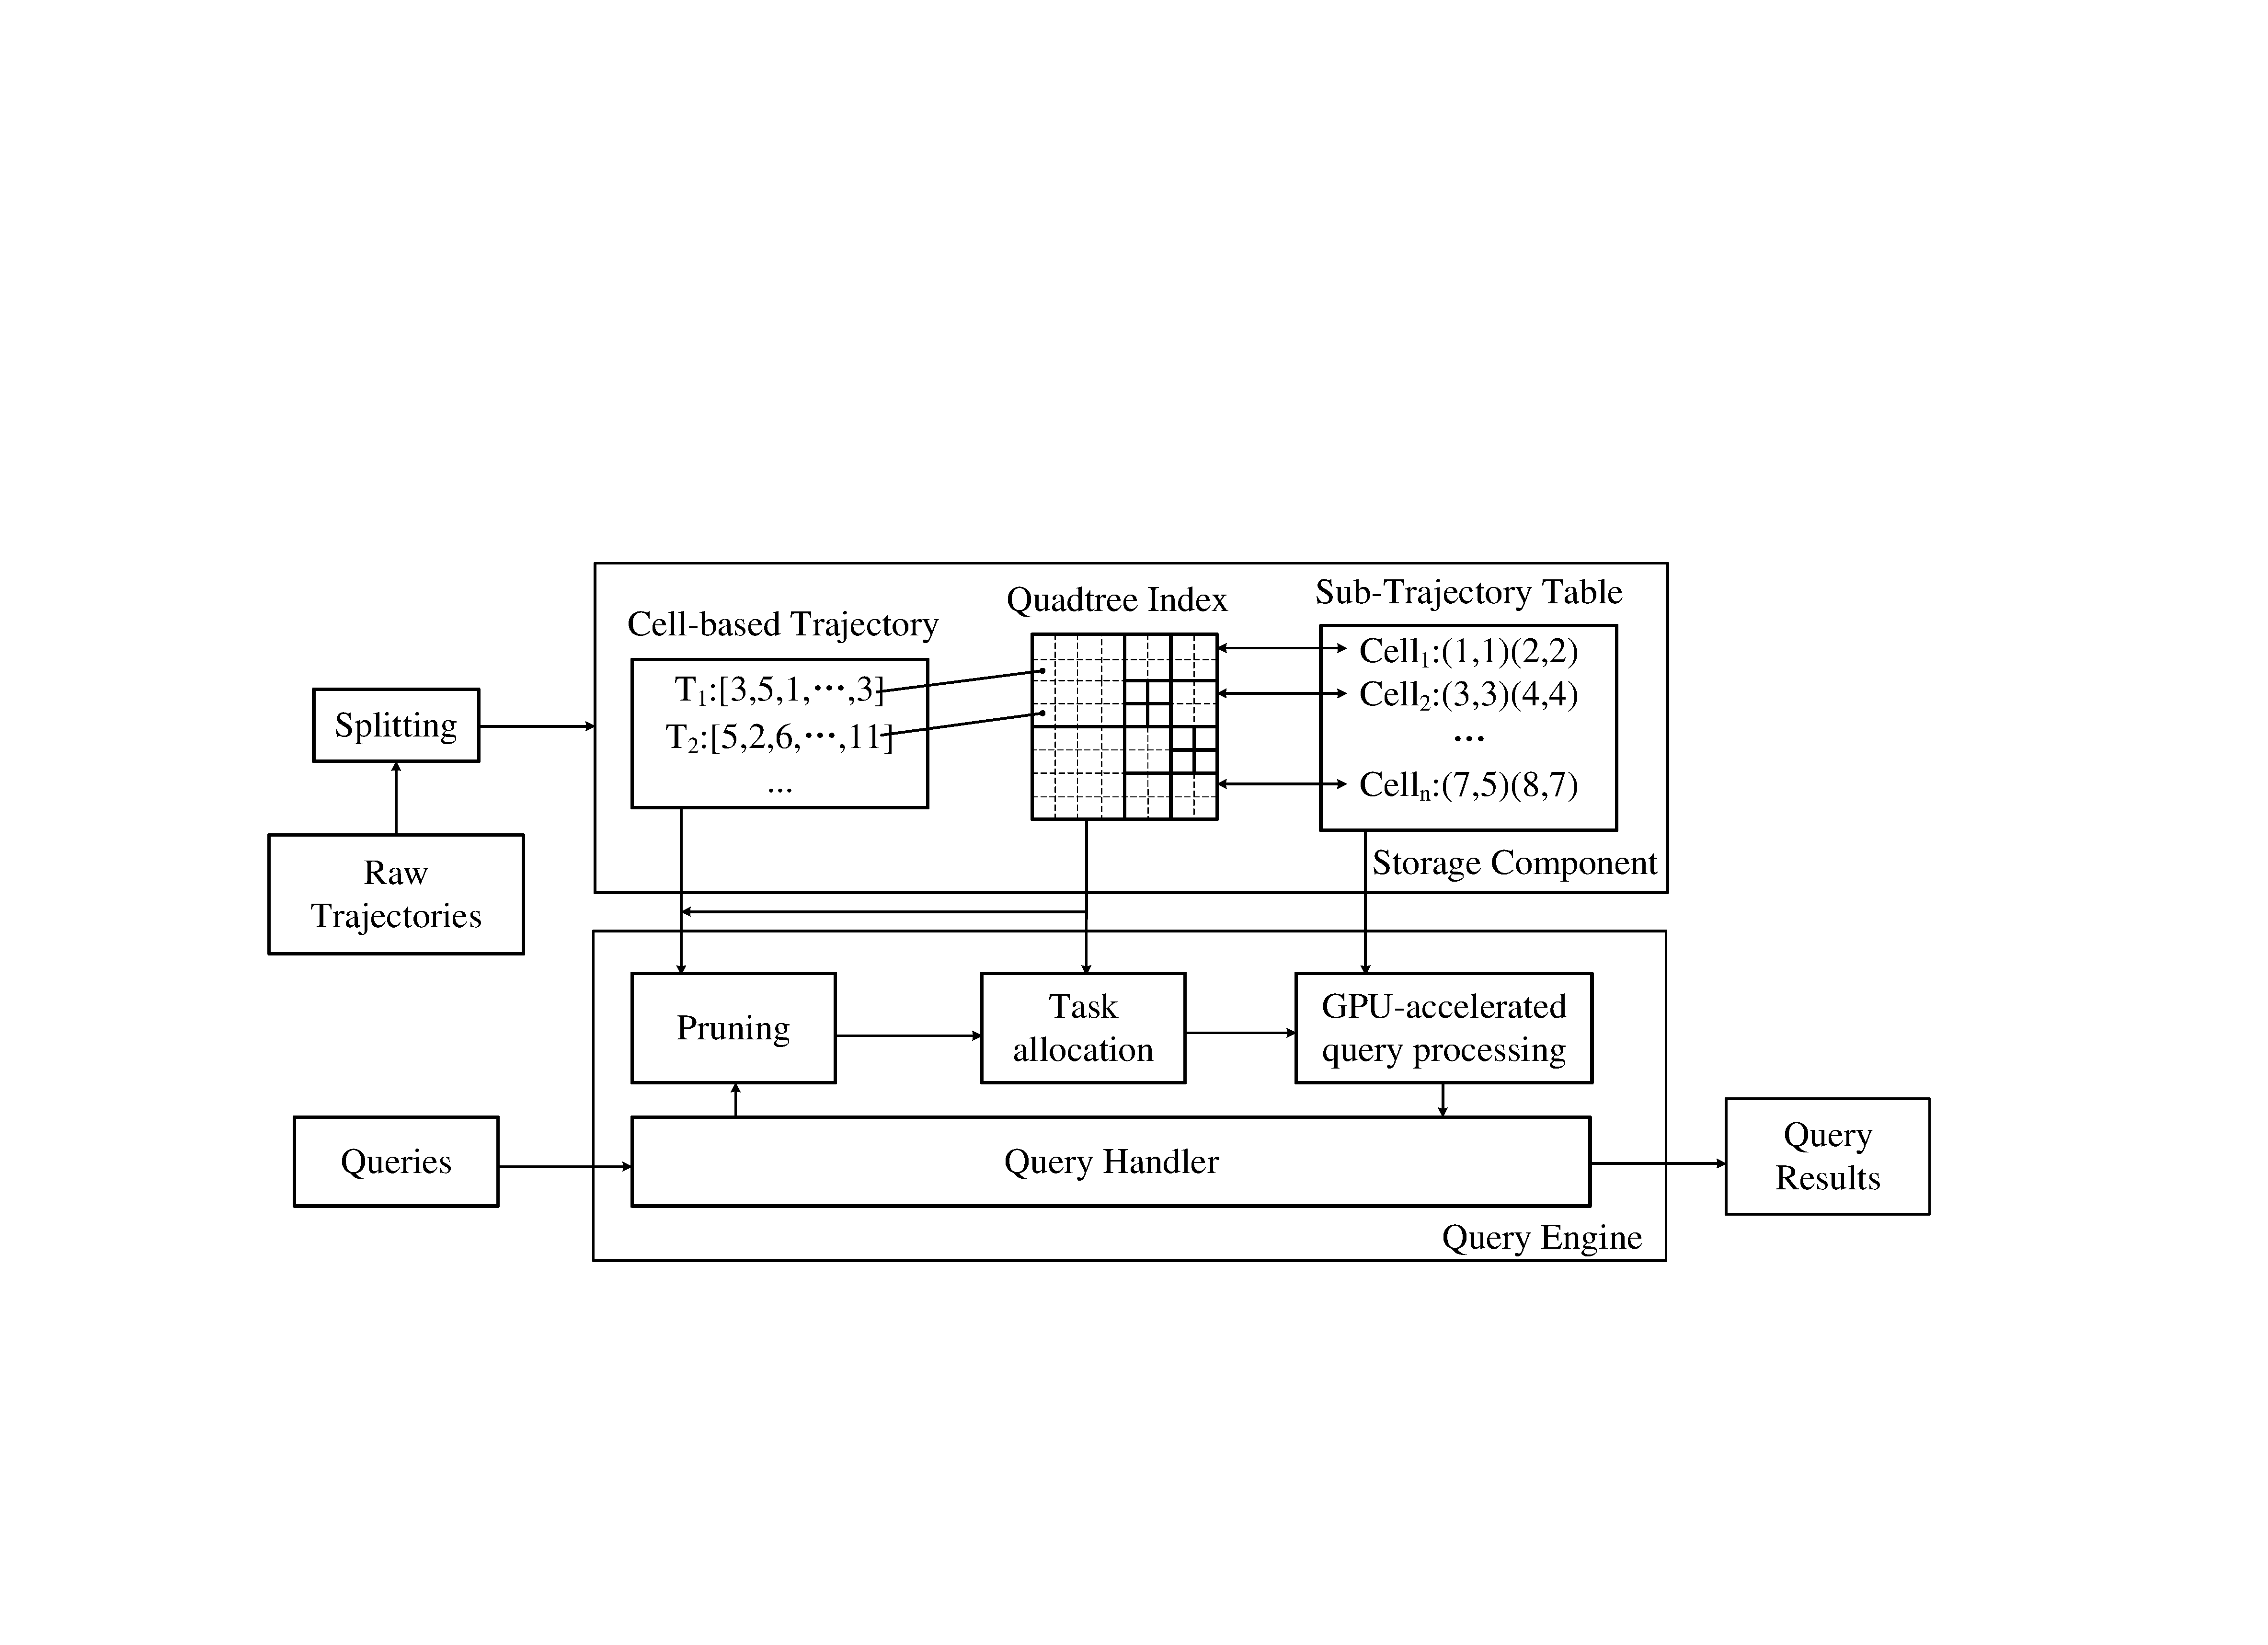
\includegraphics[width=16cm]{pdf/architecture1.pdf}
	\caption{System Architecture\label{fig:Archi}}
\end{figure*}

\subsection{Storage Component}
In the design of storage component, we exploit the potential oppotunities of quadtree with Morton encoding\cite{DBLP:conf/gis/LettichOS15} with the consideration of GPGPU and propose an index called GT-quadtree. We divide all trajectories into sub-trajectories with small cell, after which each cell in quadtree is related to a set of sub-trajectories. To rebuild the whole trajectory from sub-trajectories easily, we propose a data structure named "cell-based trajectories" for each trajectory, storing the cell's identification it goes through, according to its original order. Sub-trajectories and quadtree are stored in in host memory, which is usually large enough to store the whole data. And cell-based trajectories are stored in GPU global memory, for faster parallel pruning on similarity query. The detail of storage component will be introduced in Section IV.

\subsection{Query Engine}
Our query engine is designed for handling thousands of queries including three basic kinds in parallel, optimizing for executing time per query. For different kinds of query, we first adopt different pruning strategies to reduce unneccessary computation by help of index. After that, we divide the all the queries into tasks at both coarse-grained level and fine-grained level, according to the CUDA's programming framework. We then transmit as less data to GPU, which executes produced tasks in parallel and output the query results. We will illustrate query engine in Section V.

\section{GPU-friendly Storage Component}
In this section, we first introduce the index based on Mentor encoded quadtree. After that, we propose the benefits of Mentor encoded quadtree in supportting three kinds of queries, considering the characters of GPGPU computing mentioned before. At last, we propose the construction of our index.

\subsection{Storage Design}

Index performs as an important role in storage system by pruning unneccessary accessing of data. However, existing works about index on trajectories can not be easily used to solve our problem. First, in previous researches about trajectory storage system, different kind of query need different type of index, because of different characters of pruning strategies. Pruning on range query and k-nearest neighbor point query concern more about the relation between one query location and a trajectory. On the other hand, pruning on top-k similarity query concerns about the relation between two trajectories, which are sequences of locations, make it differentiated from two kinds of queries mentioned. Second, as mentioned in background, programming framework of CUDA raises a mass of claims about storage.

Fixed grid index can be used to solve the first challenge. An example of fixed grid is shown in middle in storage component of figure \ref{fig:Archi} . Each cell has an identifier and stores the pointers linking to the sub-trajectories it contains. For top-k similarity query, an lower bound of similarity distance can be derived by a histogram method\cite{DBLP:conf/sigmod/ChenOO05}, which plays an important role in pruning strategy. In this histogram method, given the whole plane [$(x_{min},x_{max},y_{min},y_{max})$], it is divided into $\tau_{x}$ intervals in x axis and $\tau_{y}$ intervals in y axis, forming bins $\{(x_{i},x_{i+1},y_{j},y_{j+1})|1 \leq i\leq \tau_{x},1 \leq j\leq \tau_{y}\}$. For each bin, the number of points of each trajectory falling in the area of this bin is recorded. The trajectory histogram is then formed with all the bins. After that, the frequency distance between trajectories is defined on their histograms, which can generate the lower bound of EDR. Fixed grid index can store all the information in histogram. For example, in figure \ref{FreqGrid}, with the trajectory $t$ represented as line and sample points represented as points, a histogram is generated by counting the number of points in each cell, as the middle shows. The histogram information can be represented in grid like the right picture. Considering that fixed grid has been widely used as index in spatial database for range query, it is an valuable oppotunity that use fixed grid to deal with both two kinds of queries. 

\begin{figure}[htbp]
	\centering
%	\subfigure[Trajectory in grid]{
%		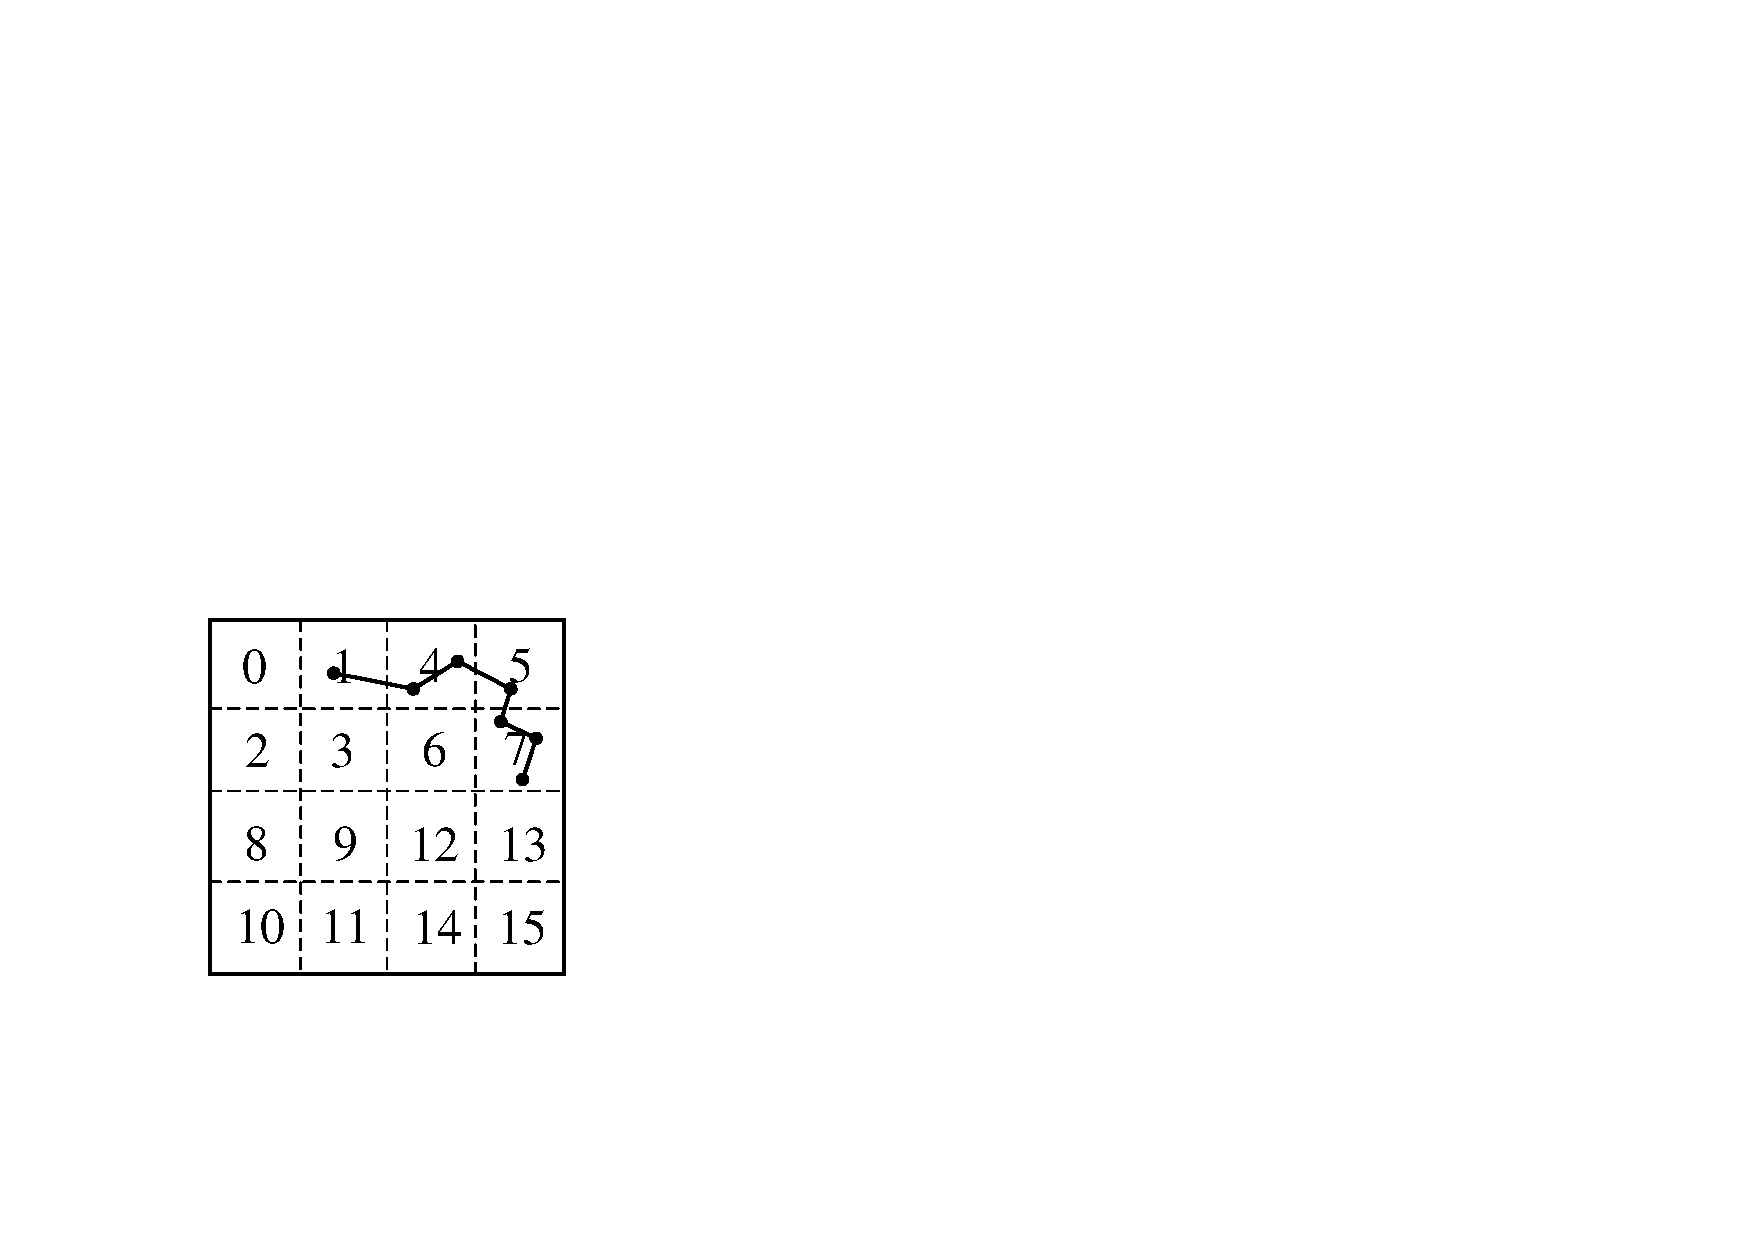
\includegraphics[width=0.9in]{pdf/Histo1}%
%		\label{TrajectoryInGrid}
%	}
%	\hfil
%	\subfigure[Histogram]{
%		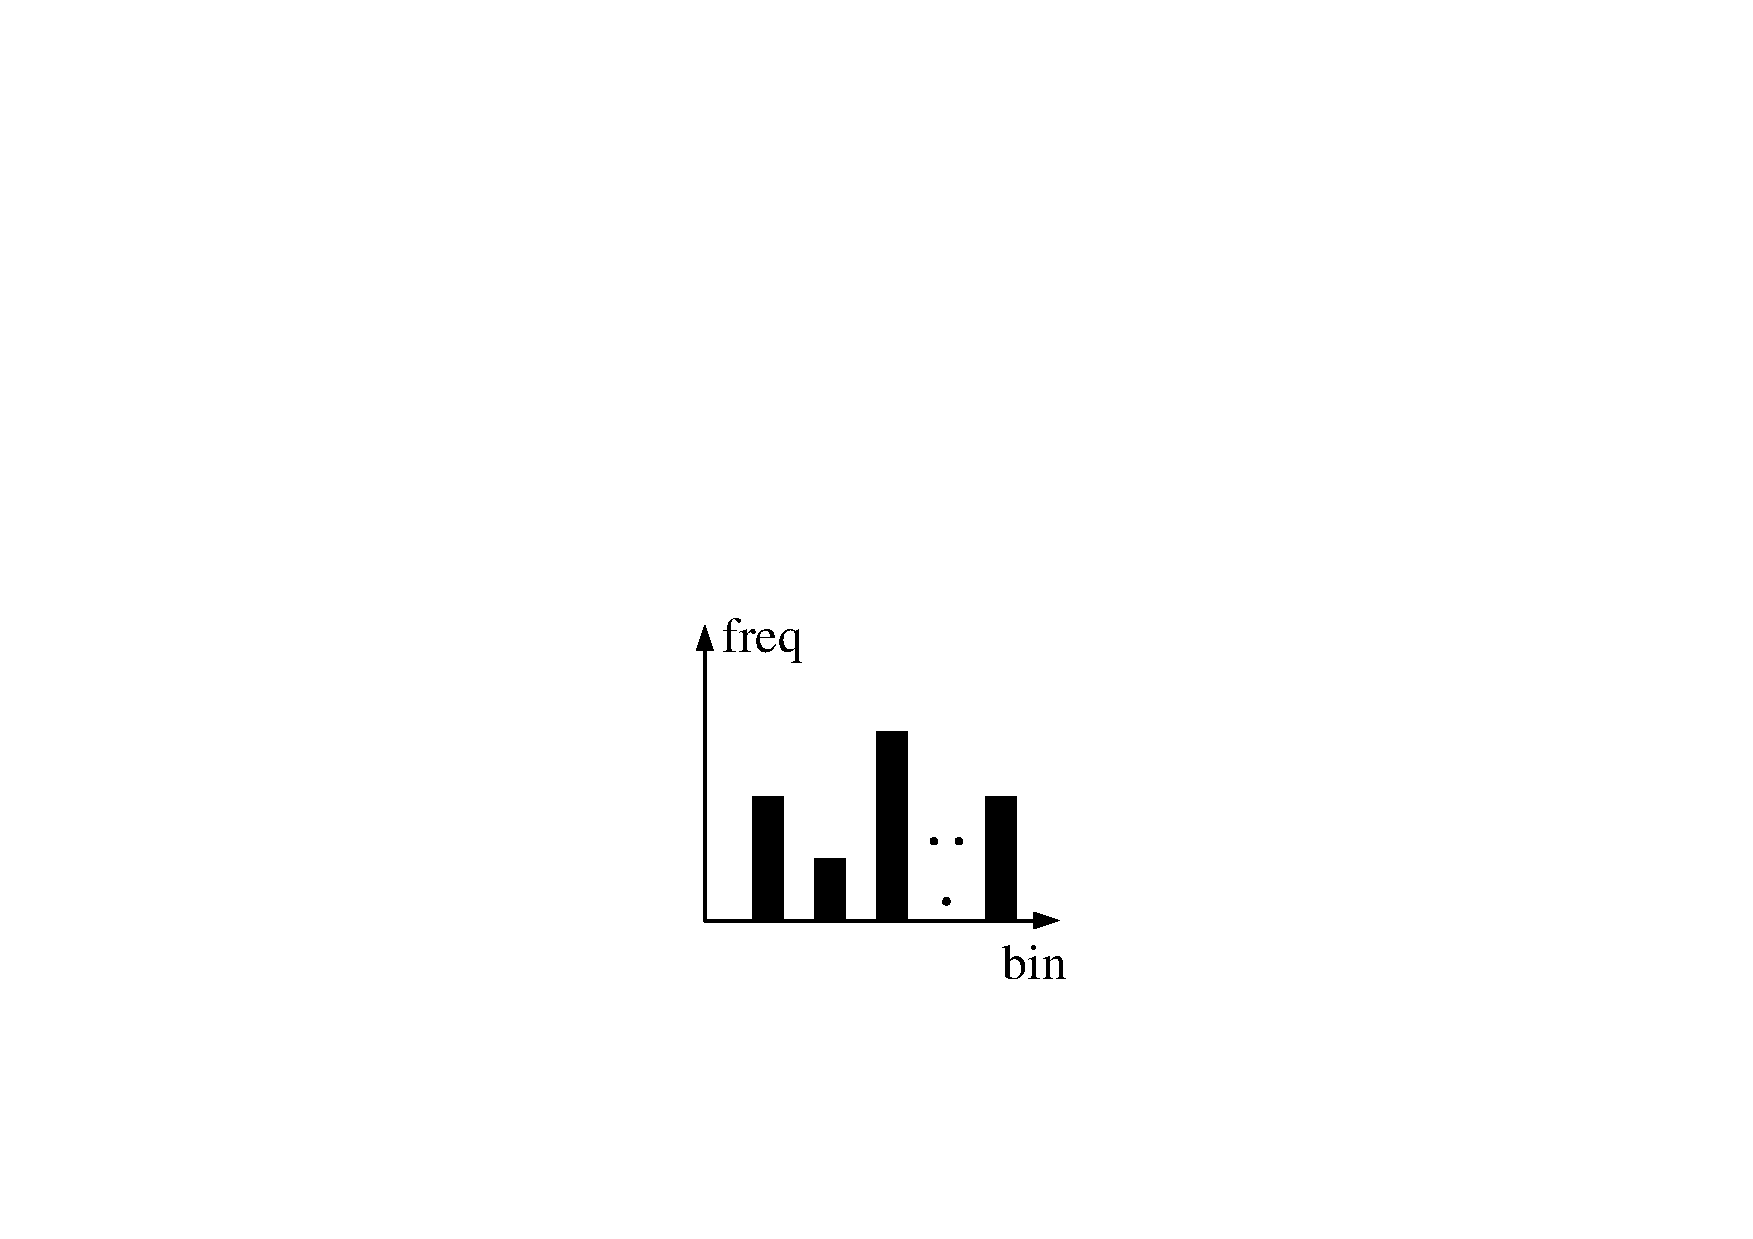
\includegraphics[width=0.9in]{pdf/Histo2}%
%		\label{Histogram}
%	}
%	\hfil
%	\subfigure[Grid]{
%		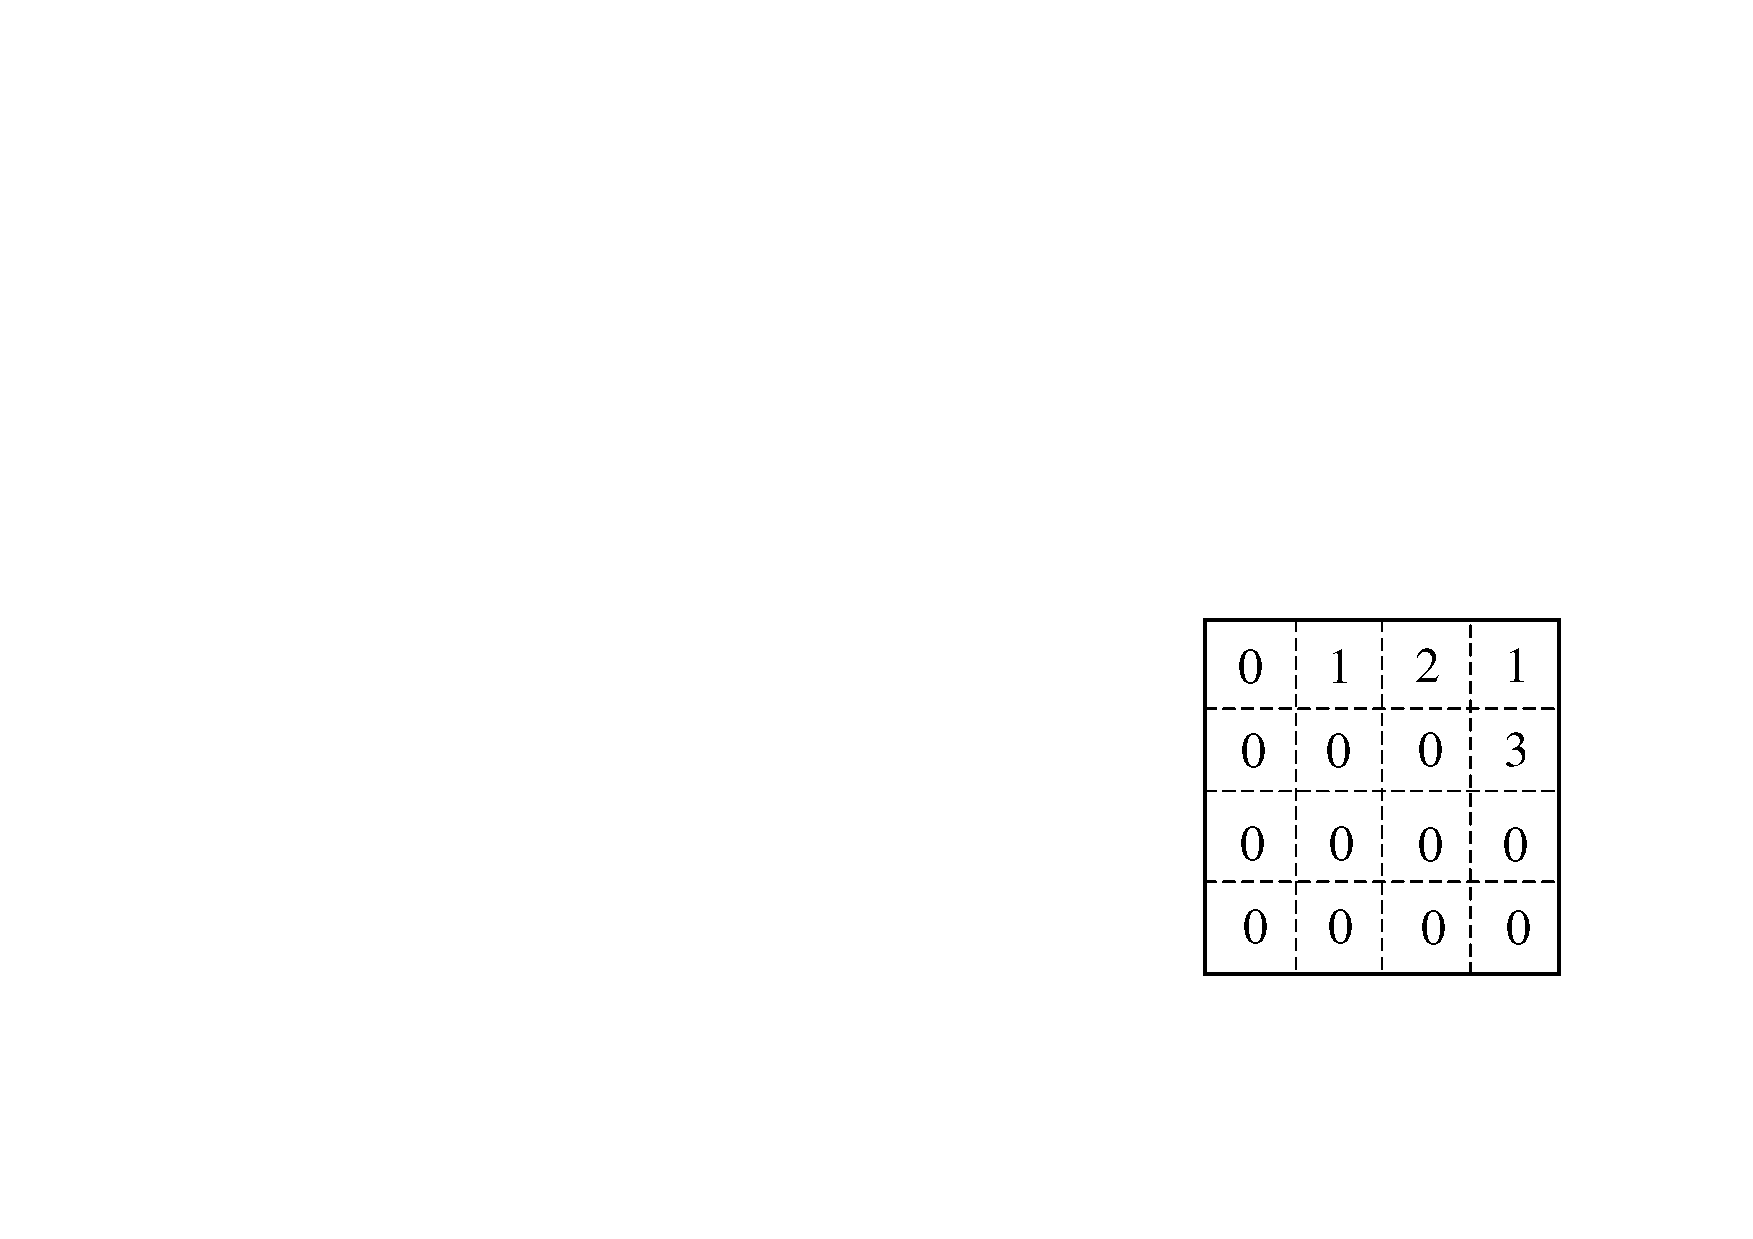
\includegraphics[width=0.9in]{pdf/Histo3}%
%		\label{FreqGrid}
%	}
	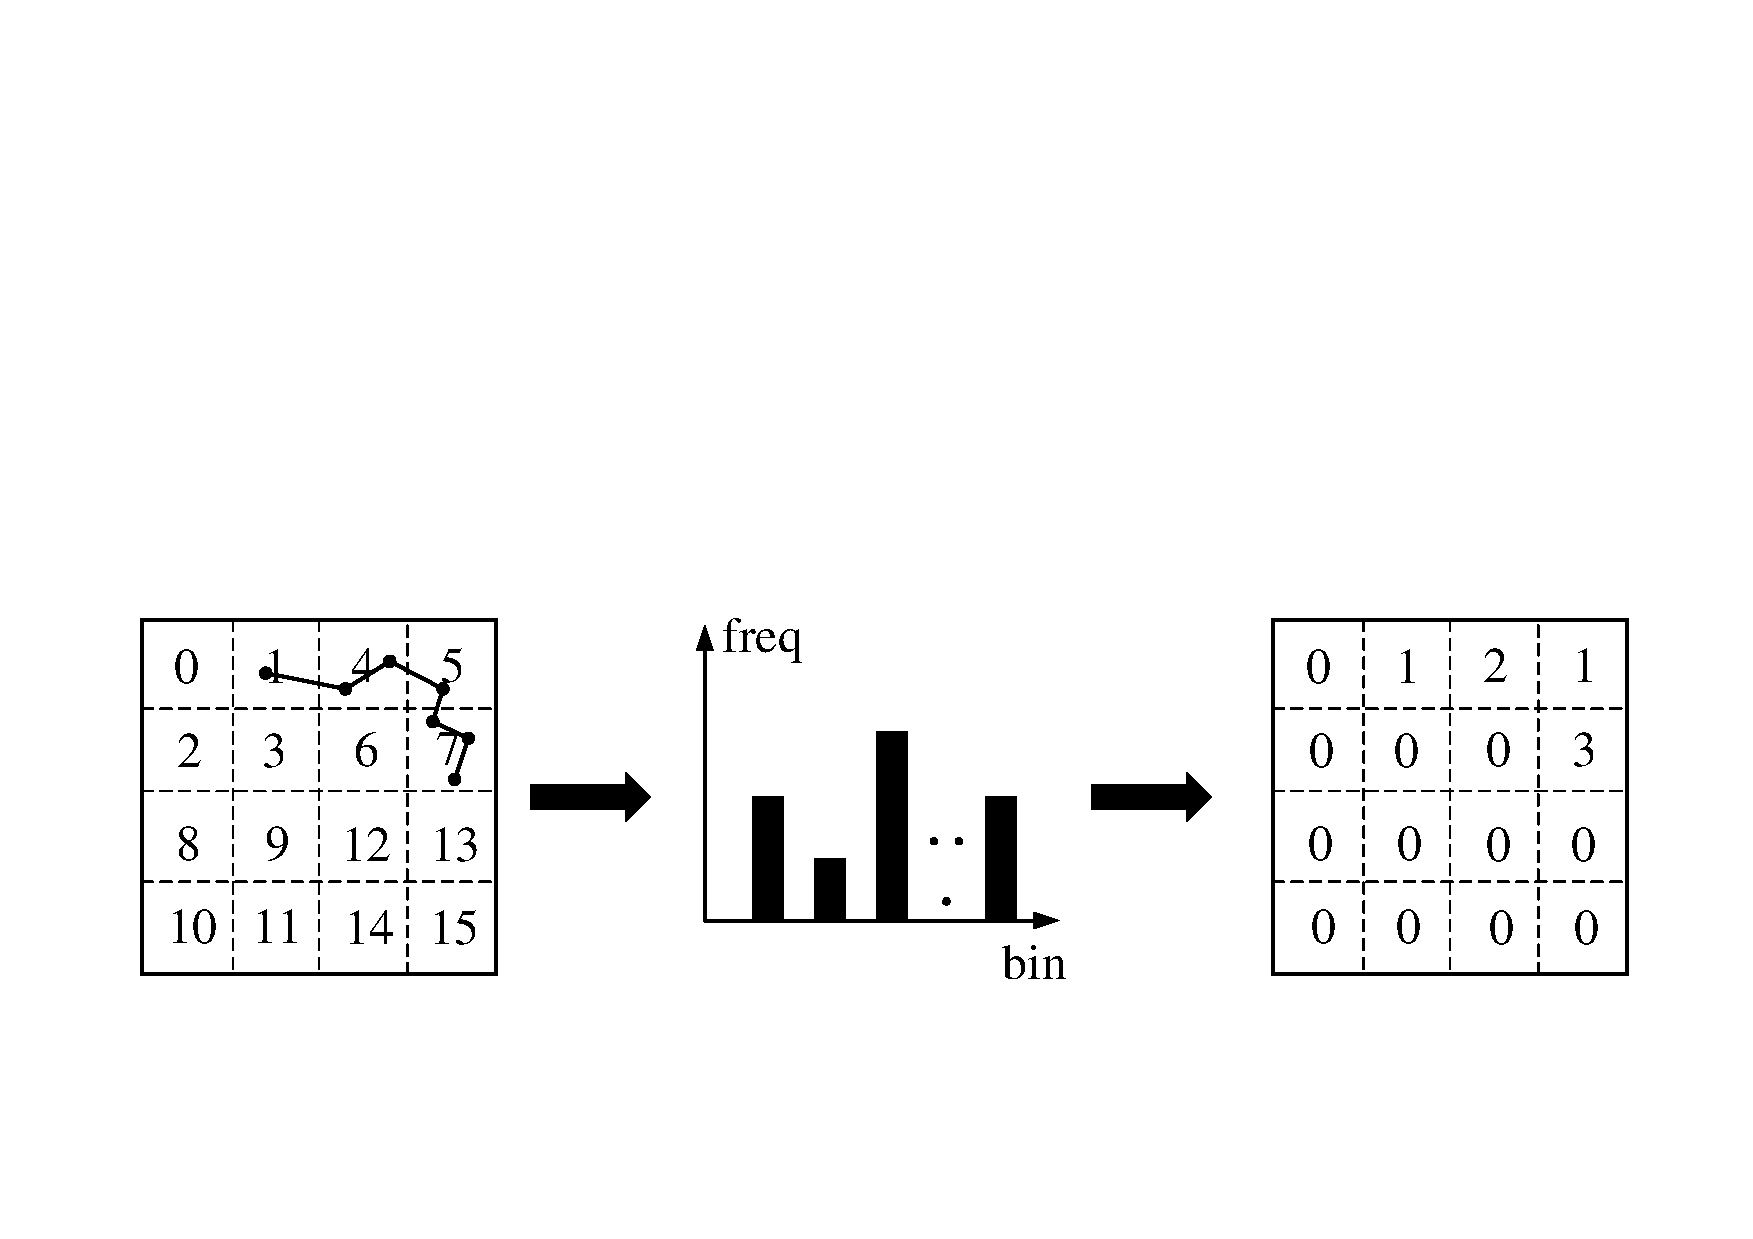
\includegraphics[width=8.7cm]{pdf/Histo.pdf}
	\caption{Example of the trajectory in area (left), the histogram of this trajectory (middle) and the grid that can represent the histogram's value (right)}
	\label{FreqGrid}
\end{figure}

However, because of the heterogeneous distribution of trajectories, fixed grid suffers from problems of load balancing when used as index for GPU-accelerated query. The number of sample points in each cell will vary largely. For example, one cell may contains too many sample points. In this situation, if we assign this cell to a thread, the other threads handling less points have to wait for this thread, which may reduce the speedup ratio of our system.

We adopt the idea of PR-quadtree\cite{DBLP:conf/gis/LettichOS15} to overcome this challenge. PR-quadtree is an index used to handle streaming k nearest neighbor (kNN) queries for objects, achieving the load balancing on GPU. However, it can not serve for pruning of similarity query because nodes of PR-quadtree is not with the same geographical size. To apply the advantages of PR-quadtree to our system, we develope GT-quadtree based on fixed grid index by absorbing some useful features of PR-quadtree. It reaches the goal of achieving load balancing on GPU, and meanwhile remains the function of serving as the index of similarity query. In GT-quadtree, each node is corresponding to different number of cells of fixed grid, overlaping different area in geographical plane. As figure (x) shows, %
%
% a figure shows the corresponding of tree and the cells
%
the root is corresponding to the whole plane. Except for root, one and another levels of nodes are generated recursively by dividing areas of their parent into four quadrant to make sure the number of points within each node's area is all less than a user specified parameter $vol_{max}$. Also, if the number of points in a node is less than $vol_{max}$, it would not be divided anymore and regarded as leaf node. GT-quadtree is built based on fixed grid, with each leaf node containing all the cells of grid within its spatial area. Morton encoded identifiers are assigned to cells of fixed grid and nodes at different levels of GT-quadtree, as figure \ref{GTQuadtree} shows, noting that the node $i$ in $j$ level is represented as $(j,i)$. With the help of Morton encoding, we can traverse from a node to its parent within a bitwise operation in GT-quadtree and vice versa. For example, in case showed in figure \ref{GTQuadtree}, the parent of node $(2,4)$ in figure \ref{NodesL12} is $(1,1)$ in figure \ref{NodesL1}. This process is done by profroming a two-bits right shift on $100(4)$, getting $1(1)$. 

%Moreover, operation judging whether two bins are adjacent, which is required in histogram pruning algorithm when doing similarity query, can be fastly finished with Morton encoding. Converting the identifier into binary, the odd number bits represent the x-coordinate and even number bits represent the y-coordinate. Figure xx shows an example,  

\begin{figure}[htbp]
	\centering
	\subfigure[Morton encoding in level 1]{
		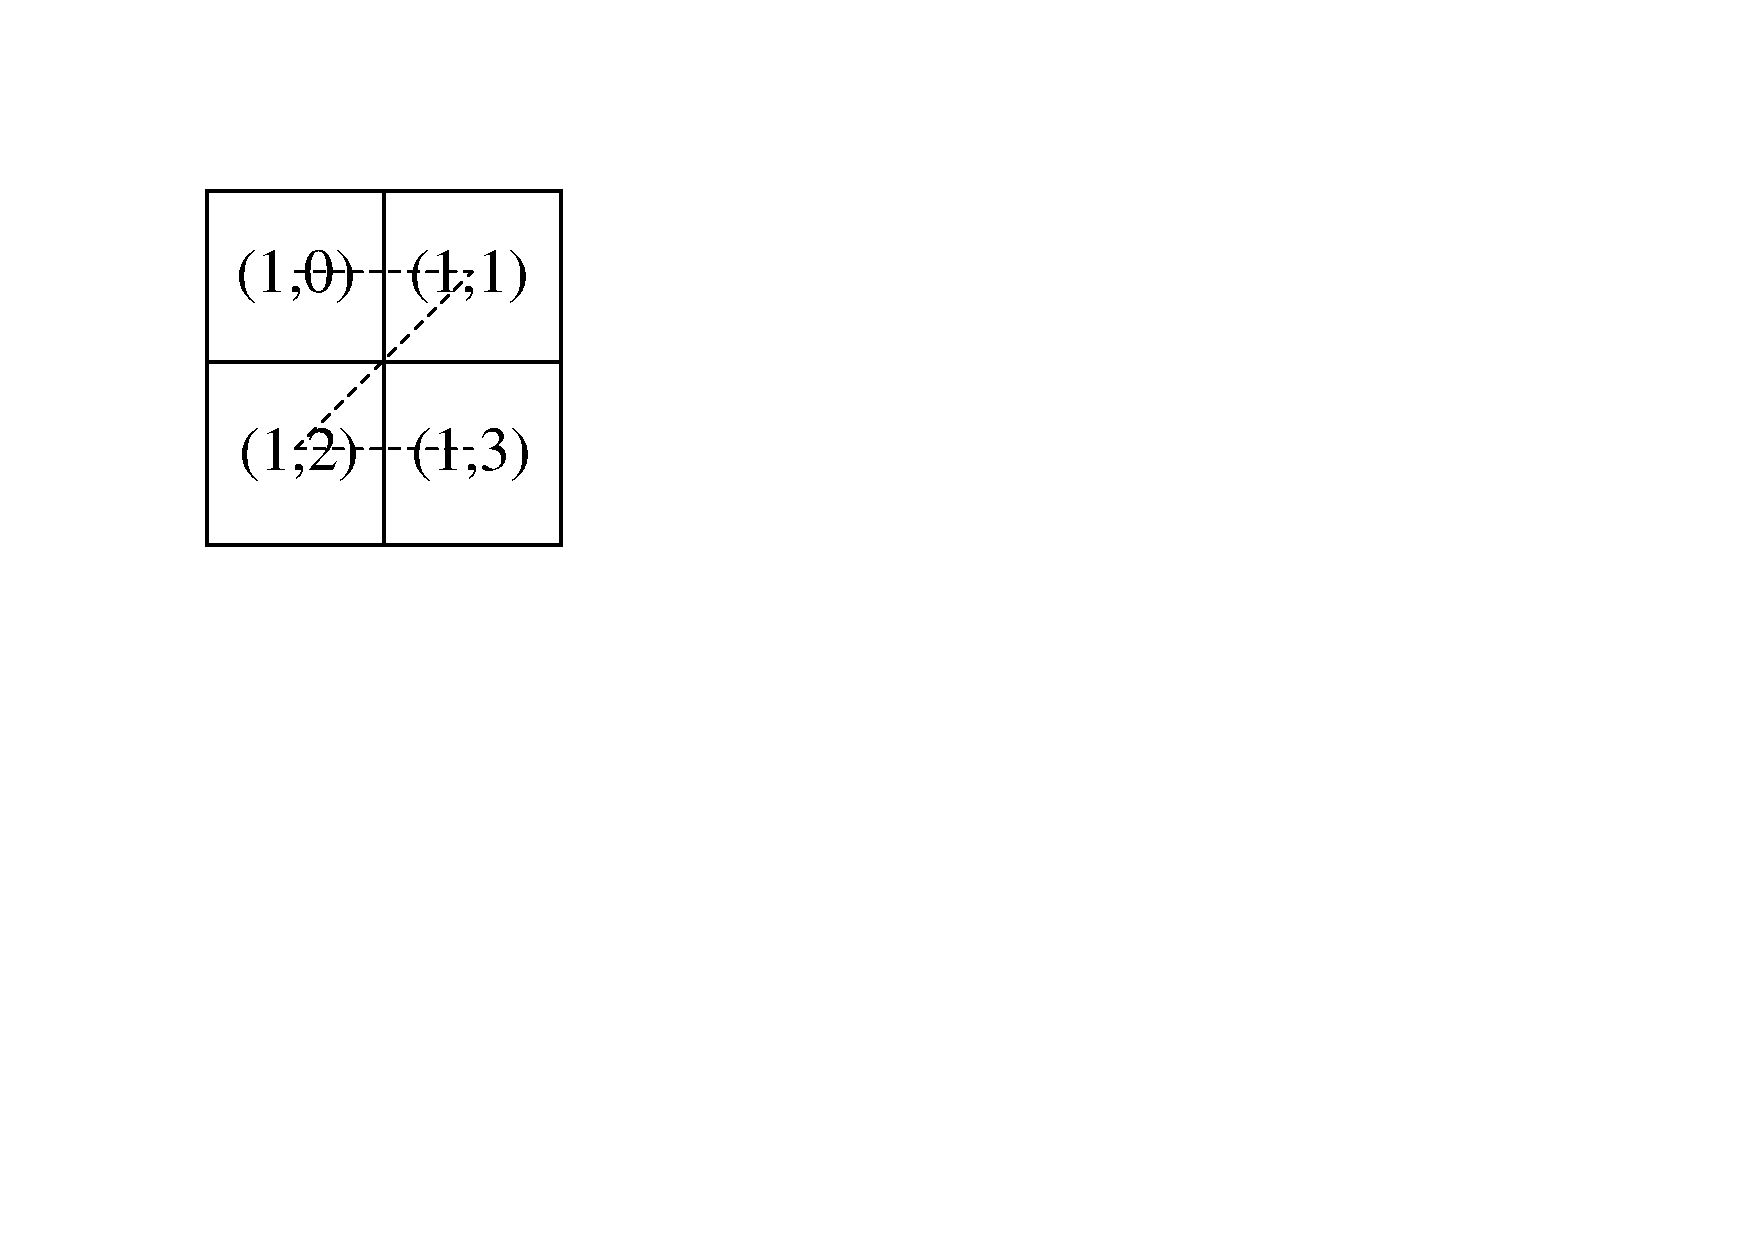
\includegraphics[width=0.9in]{pdf/GTTree1}%
		\label{NodesL1}
	}
	\hfil
	\subfigure[Morton encoding in level 1 and 2]{
		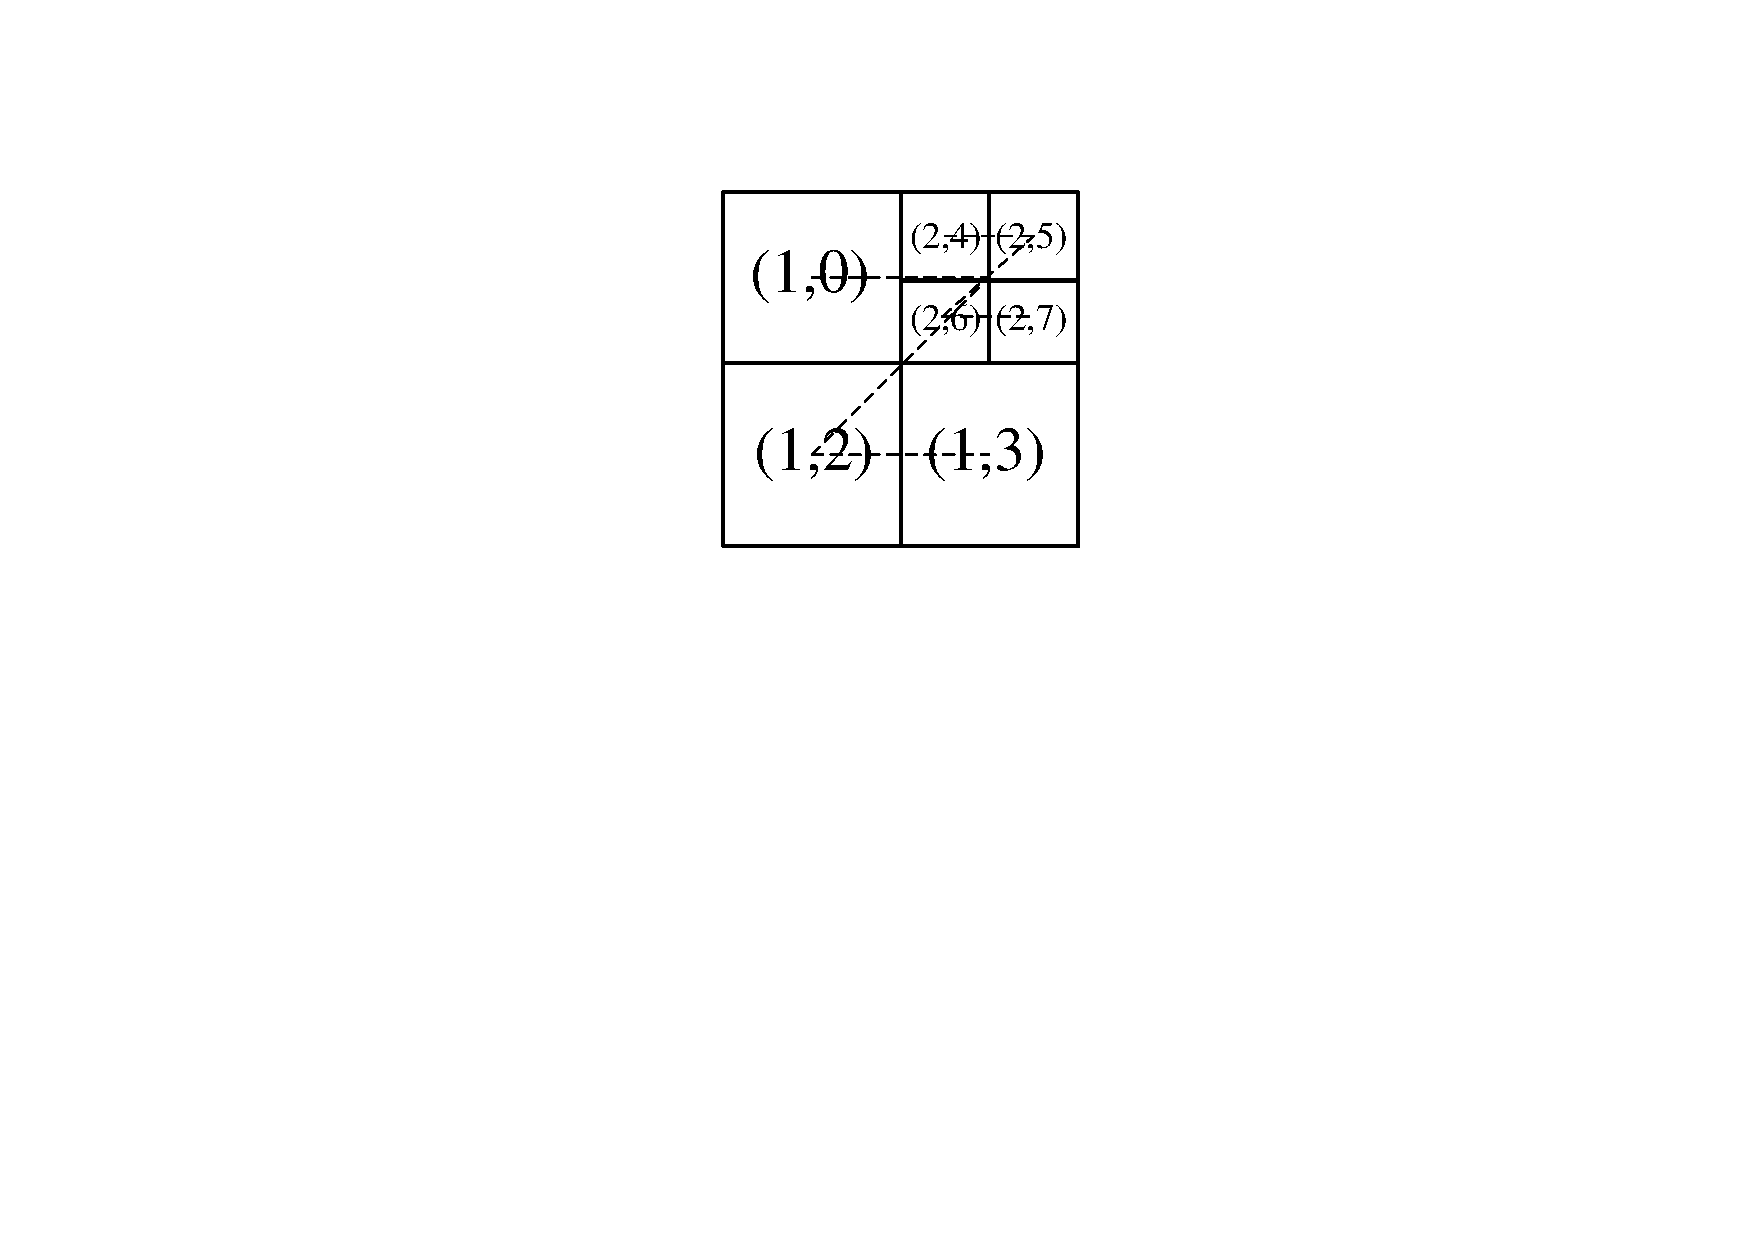
\includegraphics[width=0.9in]{pdf/GTTree2}%
		\label{NodesL12}
	}
	\hfil
	\subfigure[Morton encoding in grid of GT-quadtree]{
		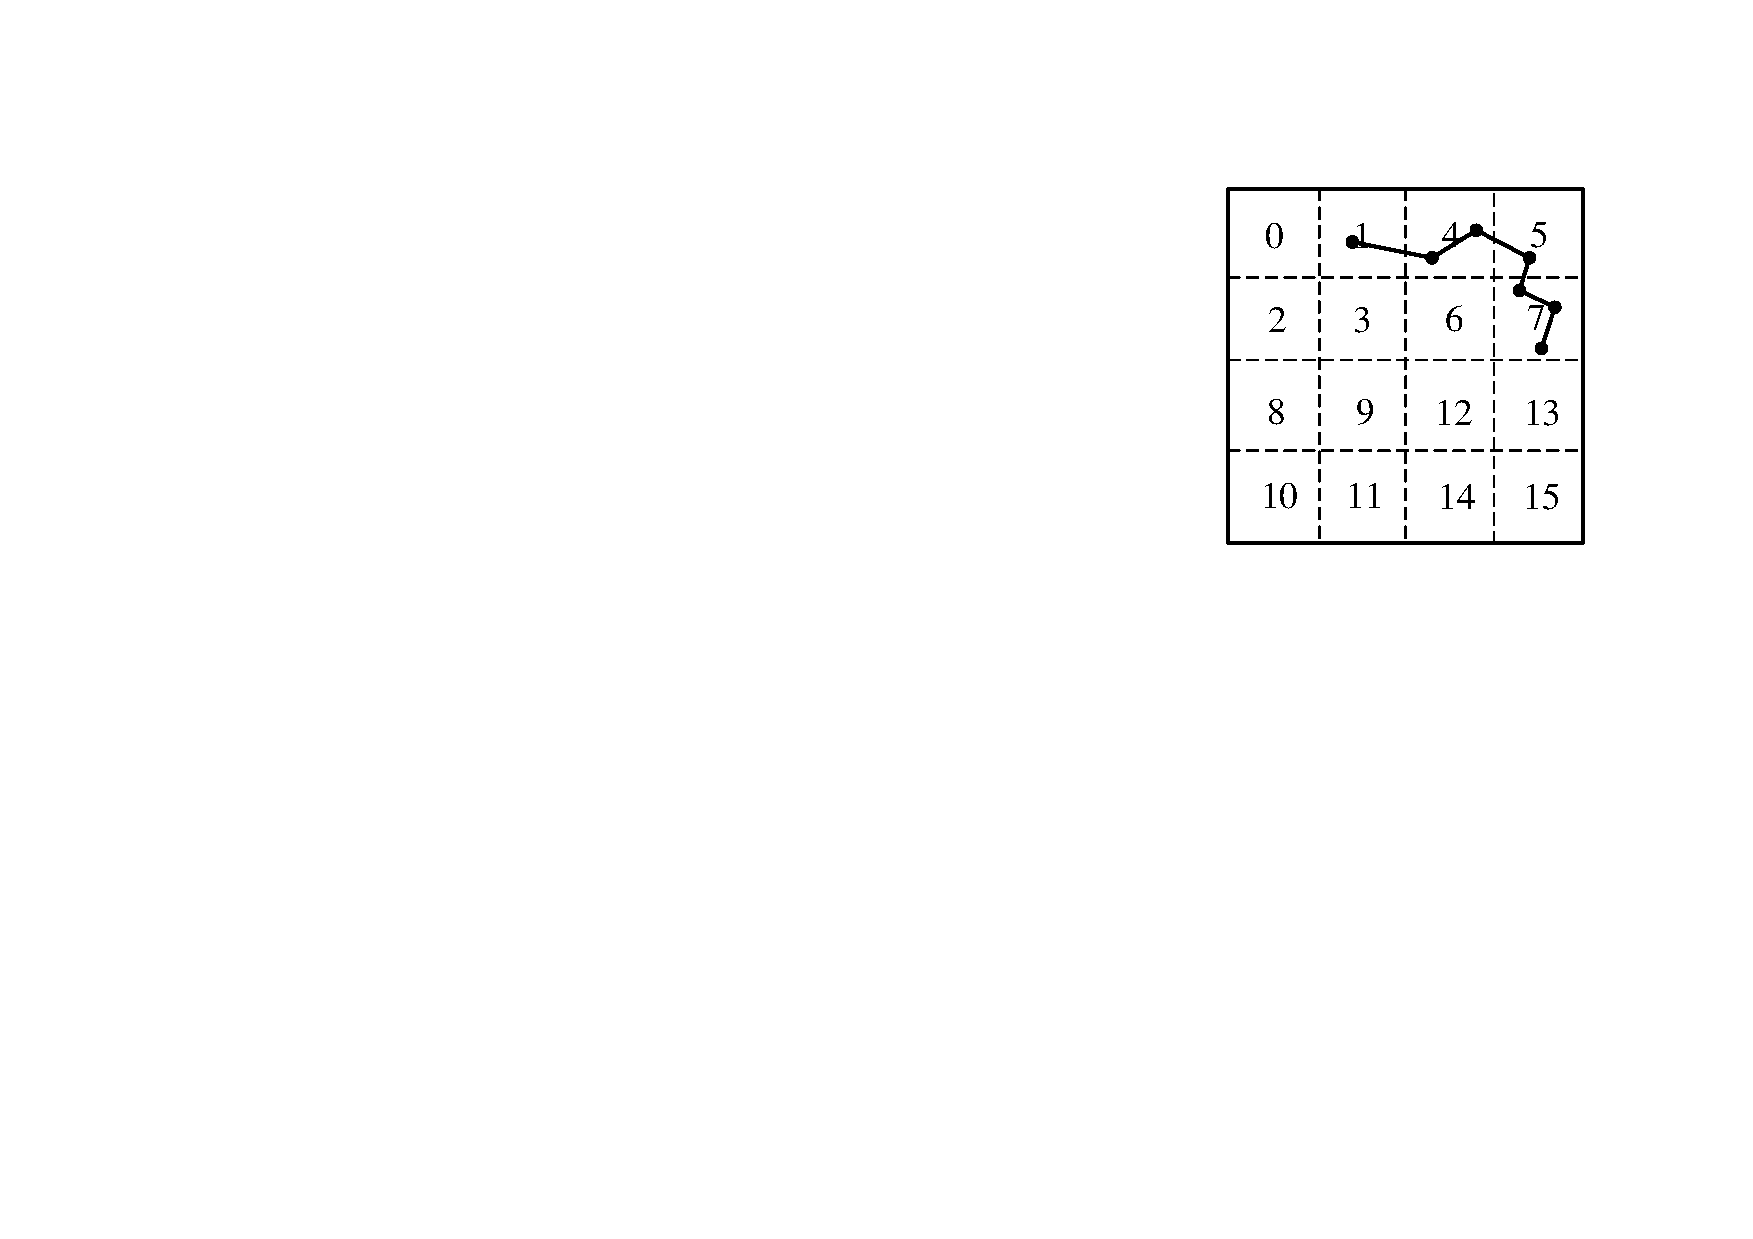
\includegraphics[width=0.9in]{pdf/GTTree3}%
		\label{Grid}
	}
	\caption{An example of Morton encoded GT-quadtree}
	\label{GTQuadtree}
\end{figure}

We designed sub-trajectories arrays storing the original geogrophical information of trajectories, making GT-quadtree meet with the memory access pattern required by GPU. Sub-trajectories array contains the sample points whose locations are within a given cell in GT-quadtree's fixed grid. These points are organized as the order of time. Meanwhile, points belong to the same trajectory are distributed together. For example, if there are sample points $\{p_{1,1},p_{1,2},...,p_{1,m}\}$ and $\{p_{2,5},p_{2,6},...,p_{2,n}\}$ from trajectory $t_{1}$ and $t_{2}$ in cell $15$, the content of sub-trajectories array of cell $15$ will be $\{p_{1,1},p_{1,2},...,p_{1,m},p_{2,5},p_{2,6},...,p_{2,n}\}$. This arrangement benifits the query performance because when the points of one cell are transferred into GPU they are located together in global memory, which satisfies the condition of coalesce accessing when GPU cores fetching data from global memory. With Morton encoding of identifiers of nodes, cells within the same node are stored continuously, indicating points within the same node are also stored continuously. \textbf{This benefit will be illustrated in detail when we introduce query engine. (Add a figure to illustrate this)}

Operation of accessing to the whole trajectory is neccessary for similarity query based on local time shifting. To satisfy this requirement, we create the cell-based trajectory list to obtain the whole trajectory with the help of sub-trajectories arrays and fixed grid of GT-quadtree. The list contains the cell-based trajectories, each of which is transformed from the original trajectory by recording all cells' identifiers it goes through as a sequence. For example, in figure \ref{GTQuadtree}, the trajectory can be transformed into its cell-based trajectory $[1,4,4,5,7,7,7]$. After this transformation, we can fetch the whole trajectory by reading the sample points from sub-trajectories array of cells in cell-based trajectory one after another. We can also generate the frequency vector of a trajectory quickly from corresponding cell-based trajectory, which plays an important role in pruning for similarity query.

\subsection{Construction}

(This part differ very small)

Storage component construction starts initially with an empty fixed grid covering the whole spatial plane. We first set the length of each cell is set to $m$ times of specified noise threshold of EDR distance $\epsilon$. It make the cell equivelent as two-dimensional bin. Then we build a grid containing $4^{m}$ cells, to guarantee that we can build a quadtree on it. Identifiers of cells are assigned according to the rule of Morton encoding, as figure \ref{Grid} shows.

After that, we split the input trajectories into sub-trajectories. For each trajectory, we allocate sample points to corresponding cell of the grid, in order of cell's identify one by one. Sample points within the same cell are stored continuously in sub-trajectory array, with the offsets of each trajectories are marked in the cell. In this process, we record the sequence of cells allocated, generating the cell-based trajectory. We transfer all cell-based trajectories to GPU global memory, forming the cell-based trajectory list. 

Based on this fixed grid, similar with the method in \cite{DBLP:conf/gis/LettichOS15}, we build a new quadtree as our final index, in which the number of each cell not exceeding a given threshold $vol_{max}$, assuring load balancing when dividing range query into multiple tasks. In the process of building quadtree, we start with creating an empty root node which covers all of the cells as the root of quadtree, identified as (0,0). Then we calculate the volumes for all nodes in quadtree, which indicates the number of sample points the node contains. We say a node contains a sample point if this point is within the cell which this node covers. Then, nodes whose volume is larger than $vol_{max}$ will be divided into four quadrants, forming the children nodes in next level, meanwhile other nodes are labeled as leaf nodes, containing less than $vol_{max}$ points. This procedure will be invoked recursively until there is no node to be divided. For example, in figure \ref{GTQuadtree}, node (1,1) in \ref{NodesL1}is divided into (2,4), (2,5), (2,6) and (2,7) in \ref{NodesL12}.





\section{GPU-accelerated Query Engine}
In this section, we introduce our query engine working on CPU-GPU hybrid environment. The goal of query engine is to handle both range queries and top-k similarity queries from thousands of clients and get speedup through executing tasks on GPU. For this two kinds of queries, we design parallel query algorithms respectively, including task division strategy and query procedure.

\subsection{Range Query}
% (This part is simple and similar with work in other works, so use several sentence to describe.)

There have been a solution\cite{GPUTaxi} leveraging GPU to handle range query based on quadtree. However, this solution is based on a fact that all the points will be transfered into GPU memory, which is not realistic at a big data scene. In our solution, by integrate a usage table technique, we can also achieve a similar speedup even if data are not all in GPU memory. 

Similar to the most of related work, we consider the combination of two levels of parallel, containing parallel within query and parallel among queries to fit with the two-level parallelism model of CUDA programming. We achieve this in two step. 

First, we filter sample points not within query ranges quickly through GT-quadtree. In this step, we first extract query's ID and their query ranges. Then, nodes in GT-quadtree whose cells are overlapped by the ranges of queries are retrieved and noted as candidate nodes, forming a mass of $\langle node, query\rangle $ pairs. It can be easily seen each candidate node should indeed be refined, for there exists at least one cell in it may include sample points within the result of range query. To prepare for the refine phase executed by GPU cores, the trajectory data within retrieved node are needed to be in GPU global memory. It is low efficient if duplicated data are transfered from host to GPU global memory, so we maintain a table recording the nodes whose data remain in GPU global memory and its corresponding pointer. Based on this technique, we first check whether the data of node are in GPU global memory. Only if neccessary, we transfer data of this node to GPU, otherwise the pointers of data are directly used to locate the required data. It is worth noting that CPU continue traversing the GT-quadtree simultaneously when transfering data, which can hide the latency caused by low-speed PCI to some extent. 

At the second step, we refine the candidates on GPU in parallel and get the final results. Each thread block is assigned with a $\langle node, query\rangle $ pair, finding out sample points in node within query's range. In each thread block, to guarantee coalesce accessing, sample points are verified in loops. As mentioned in GT-quadtree, sample points of the same node are stored continuously in global memory. For this reason, we propose an strategy that one thread looks for one point in each loop and output whether it is within range according to thread ID until all points within the node are verified. In this strategy memory request of the threads are nearby, leading to coalesce accessing. For example, in the first loop, thread 0 handles point 0, thread 1 handles point 1, ..., and so on. In addition, reminding that each node in GT-quadtree contains sample points no more than $vol_{max}$, the load balance is achieved in this step. Refinement procedure on multiple GPUs is similar, so we will not introduce it detailly because of the space limitation.


\subsection{Top-k Similarity Query}

The goal of our solution is generating the result of top-k similarity queries in a short time, leveraging the parallel power of GPU. We use EDR as the similarity measurement, which is popular and performs well in most of recent works. \cite{EDWP15}[] Our work can be migrated to other measurements whose calculation is based on dynamic programming algorithm, such as LCSS\cite{DBLP:conf/icde/VlachosGK02}. However, considering that GPU efficiency is low if the task load is small, it is suboptimal to directly migrate algorithm proposed by \cite{DBLP:conf/sigmod/ChenOO05} to GPU, because this algorithm execute only one EDR calculation after a filter phase. As a solution, we adapt this algorithm to fit with GPU architecture and design a new filter and refine scheme, which is shown in Algorithm \ref{alg:TSQ_1}. The initial idea of this scheme is filtering some trajectories which can be assured not appearing in the result to avoid unneccessary expensive EDR computing. 

First, for each query, we use cell-based trajectories to calculate the lower bounds of EDR between query trajectory and trajectories in storage and add all trajectories to candidate set (line 3-5). After that, we find $\eta$ trajectories from candidate set whose lower bounds are the lowest, calculating the real EDR between query trajectory. Obtaining the upper bound of current top-k EDR distance of trajectories efficiently is a frequent operation for pruning, so a size-k priority queue of real EDR distance is maintained to handle this operation. (line 7-8). We then prune trajectories in candidate set whose lower bound is bigger than upper bound of current top-k EDR distance safely because we can assure they will never be chosen in following iterations (line 9). We repeat this process of choosing top-$\eta$ trajectories from candidate set and pruning until candidate set is empty. Finally trajectories in the priority queue are results of this top-k similarity query.

\begin{algorithm}[htb]
	\caption{Top-k Similarity Query}
	\label{alg:TSQ_1}
	\begin{algorithmic}[1]
		\REQUIRE ~~\\
		Query Trajectory Set $Q=\{ q_{1},q_{2},...,q_{M}\}$; Historical Trajectory Data $D=\{ d_{1},d_{2},...,d_{N}\}$; Parameter $k$,$\eta$;
		\ENSURE ~~\\
		Result list for each query $Result$
		\STATE $Result \leftarrow list(array[k])$
		\FOR{$q\in Q \ \textbf{parallelly}$}
		\STATE $LB \leftarrow GenerateLowerBoundParallel(q,D)$
		\STATE $realEDR \leftarrow InitialPriorityQueue()$
		\STATE $candidateSet \leftarrow D$
		\WHILE{$candidateSet$ is not empty}
		\STATE $simiTrajID \leftarrow ChooseSmall(LB,\eta)$
		\STATE $realEDR \leftarrow CalEDRParallel(simiTrajID)$
		\STATE $candidateSet \leftarrow FiltParallel(max(realEDR),$\\$candidateSet,LB)$
		\ENDWHILE
		\STATE $Result[q] \leftarrow realEDR.topID(k)$
		\ENDFOR
	\end{algorithmic}
\end{algorithm}

There is some challenges of performance in our proposed algorithm 1. In the most setting in actual situation, the number of cells are usually large, making the computation of lower bound a time-consuming process. For example, in Shanghai private cars dataset, an area of $45\times 55 km^{2}$ is divided into $247500$ cells, if threshold $\epsilon$ in EDR is set as $100m$. Besides, although through filtering, massive expensive EDR computations are still neccessary to execute. Attention that the computation cost of EDR between two trajectories is O($mn$)(m is the length of trajectory 1 and n is the length of trajectory 2), an efficiency issue arises as the length of trajectories become longer. To overcome these challenges, we use GPU to accelerate lower bound generation and EDR calculation. However, this migration is not trivial because of the special architecture and programming model of GPU. Aiming to overcome these challenges and get better performance, we will introduce our strategies and implementation in detail at following part of this section.

\subsubsection{Lower Bound Generation}
% candidate set and priority queue, calculate lower bounds in parallel.
The lower bound of EDR can be derived from cell-based trajectories. This process is proposed in \cite{DBLP:conf/sigmod/ChenOO05}. We first generate frequency vector (FV) for each trajectory, storing the sample points the trajectory has in each cell. For example, in figure x, suppose the depth of GT-quadtree is 3. For a trajectory whose cell-based trajectory is [0,0,0,0,1,1,1,2,3,3], its frequency vector would be [4,3,1,2]. Frequency distance (FD), defined as the edit distance between two FVs, has close relationship with EDR between two corresponding trajectories. It is easy to find that insert, delete and replace operations in EDR is similar to adding one, subtracting one and subtracting one in one element then adding one in other element on FV correspondingly. But one adjacent case is special. If there is an replace operation between two adjacent elements of FV, indicating these two corresponding cells are adjacent in grid, it may cause one unneccessary operation in EDR. For example, given two FVs, $v_{1}=<1,0,0,0>$, $v_{2}=<0,1,0,0>$, and corresponding trajectories $R_{1}=(t_{1},0.9)$, $R_{2}=(t_{2},1.1)$ and $\epsilon =1$, replace operation is needed in FD but unneccessary in EDR. So, we can derive that FD is the lower bound of EDR.

Although the calculation cost of FD is lower than EDR, it still spends lots of time. There are two reasons. One is there are lots of trajectories in storage and for each of them an FD should be calculated. The other is if a small $\epsilon$ is set by user, the length of FV will be very long, causing even one FD is also computational cost. To accelerate this process, we distribute the FD computation workload of all queries to GPU evenly. To improve the throughtput of our query engine, FVs are pre-computed before the first query. When a query $q$ comes, suppose there are $N$ trajectories $t_{1},t_{2},...,t_{N}$ in storage, $N$ tasks computing FD between query trajectory and trajectories in storage are generated and each of them is assigned to a thread block, acting as the lower bound of EDR. 

Algorithm 2 shows the procedure of generate FD in each thread block. Firstly we calculate the difference between two FVs (line 1-3) in parallel. Considering the adjacent case in edit distance calculation mentioned, we reduce the difference if two elements are neighbor cell in grid of GT-quadtree (line 4-12). Given an Morton encoded cell ID, its neighbors' ID can be generated in several cheap bitwise operations by thread of GPU. Finally, FD is calculated from the difference of two FVs by a parallel addition and comparison (line 13-17). With strategy that in each parallelly loop almost an equal number of elements are assigned to each thread in an sequencial increasing order, our algorithm achieves thread level load balancing and coalesce accessing pattern. It is worth noting that this process is also load balancing in task level because all FVs have the same number of elements.

\begin{algorithm}[htb]
	\caption{GenerateLowerBound}
	\label{alg:GetLB}
	\begin{algorithmic}[1]
		\REQUIRE ~~\\
		Frequency Vector of query trajectory $qFV=[qFV_{1},qFV_{2},...]$;
		
		FV of the trajectory in task $tFV=[tFV_{1},tFV_{2},...]$;
		
		Number of cells $N_{cell}$;
		\ENSURE ~~\\
		Frequency Distance between $qFV$ and $tFV$: $FD$
		\FOR{each $i<=N_{cell}$ \textbf{parallelly}}
		\STATE $dFV[i] \leftarrow qFV[i]-tFV[i]$
		\ENDFOR
		\FOR{each $i<=N_{cell}$ \textbf{parallelly}}
		\FOR{each $j$ adjacent to $i$}
		\IF{the sign of $dFV[j]$ and $dFV[i]$ are different}
		\STATE $x \leftarrow min(|dFV[i]|,|dFV[j]|)$
		\STATE $dFV[i] \leftarrow dFV[i] + ((dFV[i]>0)-0.5)*2$
		\STATE $dFV[j] \leftarrow dFV[j] + ((dFV[j]>0)-0.5)*2$
		\ENDIF
		\ENDFOR
		\ENDFOR
		\FOR{each $i<=N_{cell}$ \textbf{parallelly}}
		\STATE $positive \leftarrow positive+(dFV[i]>0)*dFV[i]$
		\STATE $neagtive \leftarrow negative+(dFV[i]<0)*dFV[i]$
		\ENDFOR
		\STATE $FD \leftarrow max(positive,negative)$
	\end{algorithmic}
\end{algorithm}

\subsubsection{Parallel EDR Calculatation}
% introduce how to calculate EDR in parallel on GPU
% include different size strategy, task generation, data transferring and data arrangement.
After generating lower bound and pruning, a mass of EDR calculations tasks are waited for executing. Each EDR calculation takes in two inputs trajectories $traj_1$ and $traj_2$, and output the EDR distance between them. For executing massive EDR calculations in parallel, the key is to finding an approach of dividing the each calculation process into independent sub-processes.  

We designed an iterative framework for parallel EDR calculation. The EDR calculation, which is acutually a dynamic programming, can be divided into several independent steps of comparisons. Figure \ref{fig:DPstate} shows an example of calculating the EDR  between two trajectorie $traj_1$ and $traj_2$ with length $m$ and $n$. Each value in a state (represented as $state[i][j]$) is calculated by comparing and choosing the minimun value of $\{state[i-1][j]+1,state[i][j-1]+1,state[i-1][j-1]+subcost\}$, according the definition of EDR in section 2. After all the states have been calculated, the $state[m][n]$ is the EDR between two trajectories. If we use slashes to group the states, we notice that the values of states in one slash rely on the value of states in two upper left slashes. For example, in figure \ref{fig:DPstate}, if we want to calculate the states on slash 3, the states on slash 1 and slash 2 are needed. Meanwhile, comparing operations within a slash have no relationship, inspiring us to invoke the calculations within the same slash in parallel, forming the basic idea of our solution.

Based on this framework, we propose a procedure of calculating EDRs in parallel on GPU, as algorithm \ref{alg:EDR} shows, whose implement is based on CUDA. Given a set of EDR calculation tasks, we first assign each of them to a block to make GPU full-loading, in order to improve the throughtput(line 1-2). In each block, the values of states are calculated in $(2\times max\{m,n\}+1)$ loops from $state[0][0]$ to $state[m][n]$ slash by slash (line 10). For example, in figure \ref{fig:DPstate}, state on slash 1 is generated, and then slash 2, slash 3, ..., until the slash $(2m+1)$. In each loop data on two before slashes are stored in high-speed local memory of each SM, which is allocated before starting loops (line 6), because they will be frequently accessed by threads. Noting that the length of trajectory is almost smaller than 2048, it is enough for space of local memory to store these data. As for the state matrix of this calculation, we store them according to the order of slash, as figure \ref{fig:DPstate} shows. In this case, the data required by threads are nearby, assuring the coalesce accessing pattern.


\begin{figure}[!t]\centering
	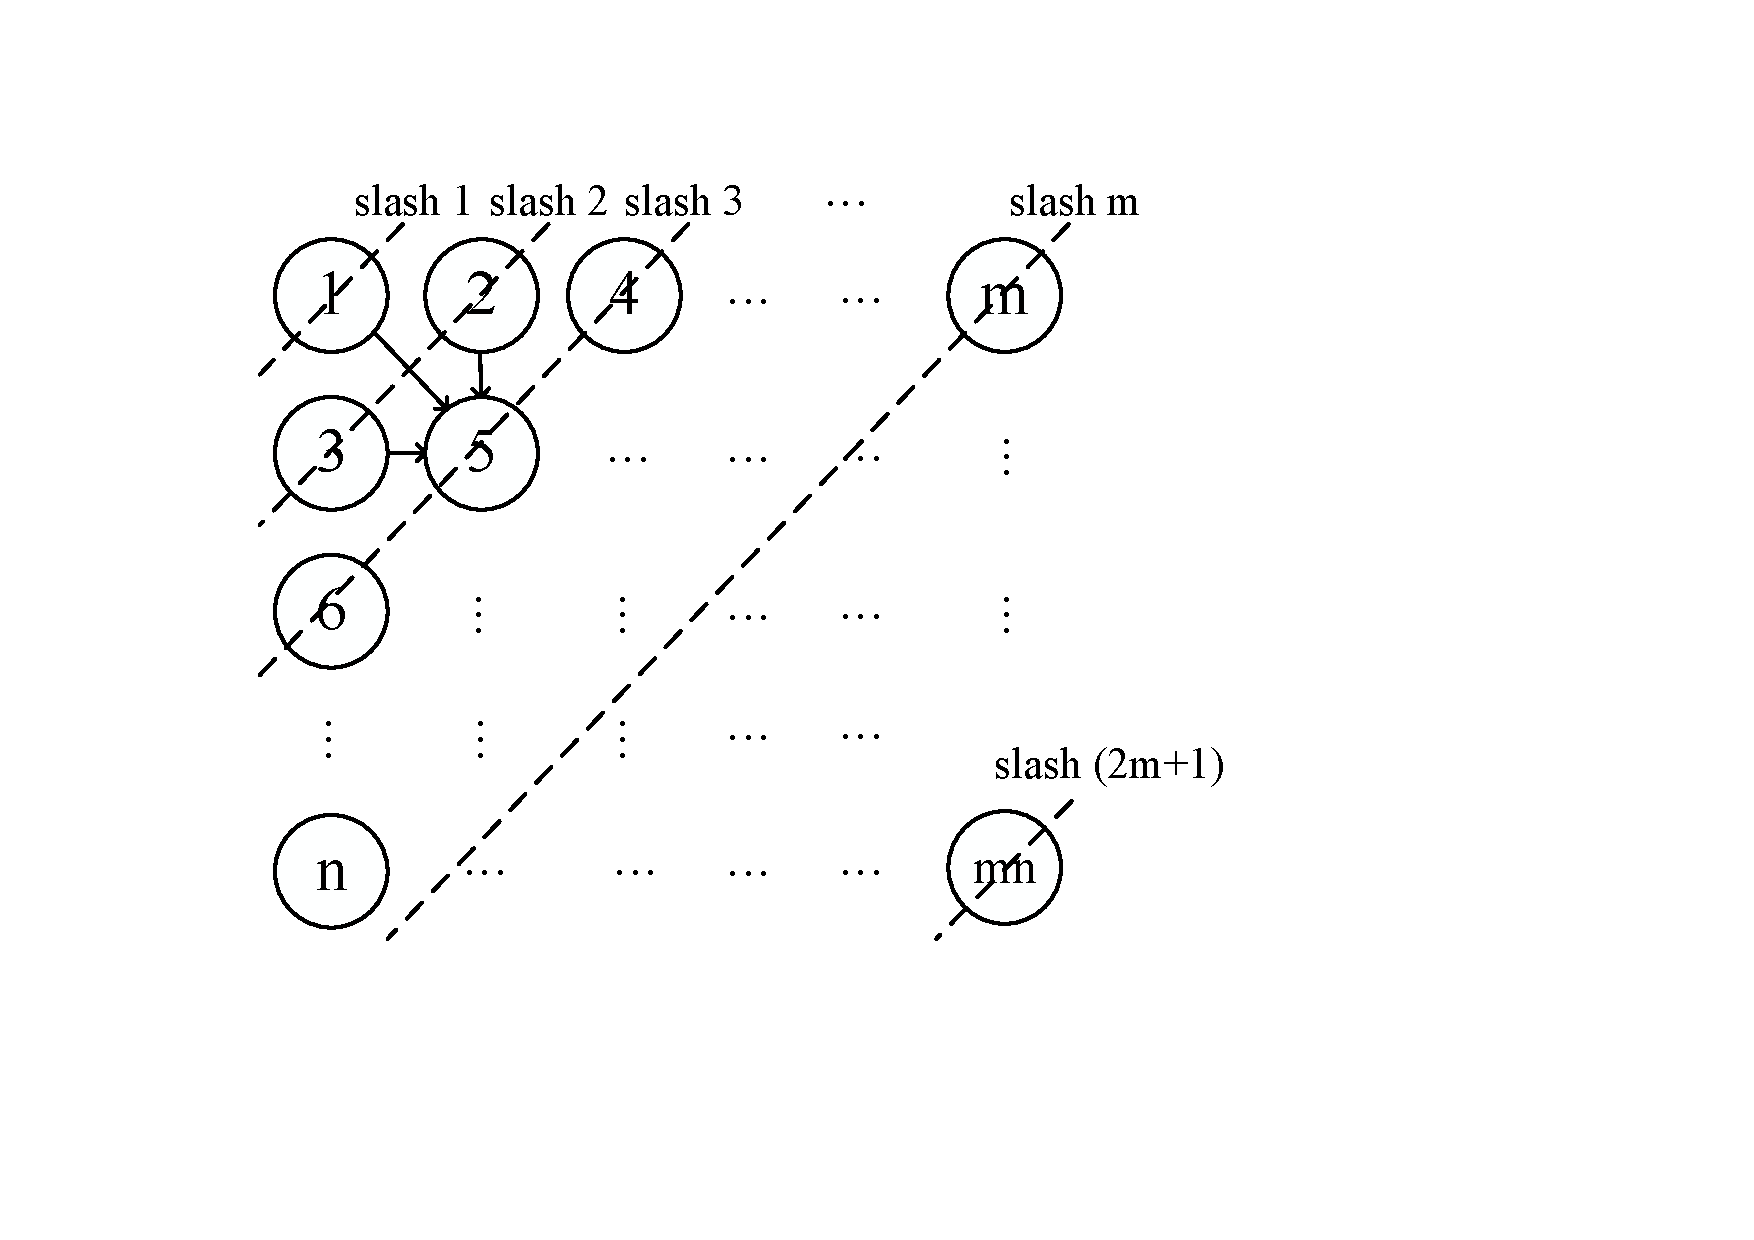
\includegraphics[width=7cm]{pdf/DPstate.pdf}
	\caption{An example of EDR calculation procedure\label{fig:DPstate}}
\end{figure}


In each thread block, based on the data of previous two slashes, all the values on current slash are calculated by mass of threads in parallel by equation (1) mentioned in Section II (line 11-16). After finishing the calculation on current slash i, the states on slash i-2 stored in local memory are flushed into state matrix in global memory, and then states on slash i-1 and i become the new "two last slashes" (line 17-22). The result of EDR calculation of this block can be extracted from state matrix after all loops (line 25). 

We can see that in our solution, the number of steps needed for EDR calculation reduces from $mn$ to $(2max\{m,n\}+1)$ comparing to not using GPU, and this reduction could be so obvious if trajectory length $m$ or $n$ is large, which is usually an actual situation because the sample interval of location device is short, e.g. 2s.

% In each loop, states in two before slashes are stored as shared variables because in CUDA programming model all shared variables will be stored in high speed local memory and calculation of states on slash $i$ is related to states on slash $(i-1)$ and $(i-2)$. In this way all of states accessing transactions required from EDR calculation are from high speed local memory. In addition to this, we find that calculation of $state[i][j]$ needs for $traj_1[i]$ and $traj_2[j]$ and in some loops all of trajectory points are required. Also storing them as shared variables is surely a choice. However, for limited capabacity of local memory, this choice will impact the efficiency of GPU. This is because in GPU architecture, each SM can execute at most 8 blocks therotically at a time but all of shared variables of blocks are needed to be resident in local memory. So abusement of shared variables may limit the number of blocks running on an SM at the same time. For this reason, we choose 

\begin{algorithm}[htb]
	\caption{Parallel EDR Calculation}
	\label{alg:EDR}
	\begin{algorithmic}[1]
		\REQUIRE ~~\\
		Two sets of trajectories: $T1,T2$
		
		Threshold of EDR: $\epsilon$
		
		Parallel parameters: $blockNum$, $threadNum$
		\ENSURE ~~\\
		all EDR distance between trajectories in two sets: $EDR(t_{1},t_{2})$, $\forall (t_{1},t_{2})\in T1\times T2$
		
		\STATE assign each $(t_1,t_2)$ pair to a thread block
		\STATE initial an array to store results of all pairs assigned: $result[blockNum]$
		\FOR{each block $bID$ \textbf{parallelly}}
			\STATE initial a matrix in global memory to store all states: $state[len(t_1)+1][len(t_2)+1]$
			\STATE $maxLength \leftarrow max(len(t_1),len(t_2))$
			\STATE initial a matrix in local memory to store states in last two slashes: $lastTwoSlash[2][maxLength+1]$
			\STATE $lastTwoSlash[0][0]=0$
			\STATE $slashNum \leftarrow len(t_1)+len(t_2)-1$
			\STATE $loopPerThread \leftarrow \lceil maxLength/threadNum\rceil$
			\FOR{each slash $i$, $i\in [1,slashNum]$}
				\FOR{each thread $tID$ \textbf{parallelly}}
					\STATE initial an array in GPU SM's register to store states calculated: $tempState[loopPerThread]$
					\FOR{each loop $j$, $j\in [0,loopPerThread-1]$}
						\STATE update $tempState[j*threadNum+tID]$ using states on last two slashes
					\ENDFOR
				\ENDFOR
				\FOR{each thread $tID$ \textbf{parallelly}}
					\FOR{each loop $j$, $j\in [0,loopPerThread-1]$}
						\STATE flush $lastTwoSlash[0][j*threadNum+tID]$ to $state$ in corresponding position
						\STATE $lastTwoSlash[0][j*threadNum+tID]\leftarrow lastTwoSlash[1][j*threadNum+tID]$
						\STATE update $lastTwoSlash[1][j*threadNum+tID]$ using $tempState[j]$
					\ENDFOR
				\ENDFOR
			\ENDFOR
			\STATE $result[bID]\leftarrow state[len(t_1)][len(t_2)]$
		\ENDFOR
	\end{algorithmic}
\end{algorithm}


%% 这部分是多个kernel并行,可以实现出来试试,然后加上多GPU????
%% 这部分是多个kernel并行,可以实现出来试试,然后加上多GPU????
%% 这部分是多个kernel并行,可以实现出来试试,然后加上多GPU????
We propose a multi-GPU implementation of our strategy dealing with large-scale of EDR calculation from all top-k trajectory queries by dividing the set of EDR calculation tasks into several equal size part, to achieve a load balancing and maximum usage of multiple GPUs. Before running these tasks, we use an independent memory allocated table (MAT) to store trajectory data when they are loaded into GPU global memory first, because in this way if a trajectory has been loaded into global memory, by looking for MAT we can avoid the duplicated low-speed data transfering between memory and GPU. However, the volume of the GPU global memory is usually so limited that not all trajectory data can be filled into it. To make an tradeoff, we maintain a memory pool and integrate it to MAT. If the pool is full, we use Least Recently Used (LRU) algorithm to drop some outdated trajectories. This strategy is efficient in real life because there exists hotspot within queries. For example, trajectories in city center may be required by queries more frequently because the population in city center is denser than rural area. After the kernel finishing, EDR calculation results from different GPUs are collected and query engine then filters the candidates, as shown in line 9 in algorithm \ref{alg:TSQ_1}. 


\section{Experiment}
In this section, we conduct a multiview experiment based on two real trajectory datasets to verify the performance of GTS. We first introduce the experimental environment, then evaluate the efficiency and scalability of index, and compare the performance of two kinds of queries with baseline and state-of-the-art works at last.
 
\subsection{Environment}
\subsubsection{Dataset}
We use two real life trajectories datasets to test the performance in different trajectories distribution. The first is Shanghai Private Car Data, containing xxx trajectorys of private cars in Shanghai collected from July, 2014 to April, 2015. The sampling rate...  The size of the whole data is xxxGB. The second trajectory dataset is Geolife, the data collected by ....

\subsubsection{Data Preprocessing}
In our experiment, we seem the sequence of sample points of a single car as a trajectory. If the time stamp of one point is over 30 minutes later than one before in a trajectory, we call this point a "gap". We split the trajectory into several new trajectories according to these gaps. This is because we usually only concern about the trajectory of a single route especially when handling similarity query, and trajectory with these gaps is usually not a meaningful single route. For example, a trajectory of a single car may include sample points from home to office and ones from office to home, and after spliting it two meaningful trajectories can be generated. After processing we get at total xxx.....



\subsubsection{Parameters}

To systematically test the performance of our system, we conduct our experiments under various parameter settings. Table \ref{table_param} shows the range and default value of parameters we test in experiments. For range query, there are four parameters affecting the performance. In real life, queries from users vary from area, so we test for different size of MBB in range query. We also test the situations of different number of queries to evaluate the scalability of GTS. For top-k similarity search, the execution time under different k value and number of queries are recorded. As we show in section V the length of trajectory determines the complexity of EDR calculations so we test for different length to see whether GTS gets high performance at different situation. Size of cells are altered in all of experiments of both two kinds of queries.

\begin{table}[!t]
	% increase table row spacing, adjust to taste
	\renewcommand{\arraystretch}{1.3}
	% if using array.sty, it might be a good idea to tweak the value of
	% \extrarowheight as needed to properly center the text within the cells
	\caption{Parameters ranges and default values}
	\label{table_param}
	\centering
	% Some packages, such as MDW tools, offer better commands for making tables
	% than the plain LaTeX2e tabular which is used here.
	\begin{tabular}{|c||c|c|c|}
		\hline
		Parameter & Meaning & Range & Default\\
		\hline
		$L_{cell}$ & size of each cell in grid & 0.05 - 0.4 & 0.1\\
		\hline
		$M_{cell}$ & max num. of points in a cell & 256 - 4096 & 1024\\
		\hline
		$\epsilon$ & matching threshold of EDR & 1 - 50 & 15\\
		\hline
		$S_{RQ}$ & area of range query's MBR & 0.01 - 4 & 0.5\\
		\hline
		$k$ & k value of top-\textbf{k} similarity query & 8 - 128 & 32\\
		\hline
		$N_{Q}$ & num. of queries & 256 - 8192 & 1024\\
		\hline
		$L_{QT}$ & length of query trajectory & 256 - 8192 & 1024\\
		\hline
	\end{tabular}
\end{table}

\subsubsection{Compared baselines and systems}

For range query, we implement two state-of-the-art systems supporting range query on GPU: STIG\cite{7498315} and the work of Zhang which using GPU to accelerate sparial query preocessing on big taxi trip data, noted as WOZ\cite{GPUTaxi}. However, these two systems are designed facing to spatial-temporal points rather than trajectories, so we add a data field in each point to represent the trajectory ID of it. To show the acceleration performance, we also implement CPU version GTS as the baseline method.

For similarity query, we only implement the original EDR based top-k similarity query algorithm proposed in \cite{DBLP:conf/sigmod/ChenOO05} on CPU as the baseline because as far as we know we are first to utilize GPU to accelerate EDR based top-k similarity query. All of the queries are executed for 10 times and averages of the time consuming are recorded. 


\subsubsection{Experiment Overview}

We first test the memory comsumption of our system. We measure the average and highest memory usage of different system. The memory consumption is measured after finishing building index for different size dataset, to show that our system use a similar amount of memory comparing to systems not supporting local time shifting based top-k similarity query. All other parameters are tuned to the optimal case.

After that, the scalability is tested. As there is no method to shut some cores in GPU, we can only test the situation with different number of GPUs.

In query performance part, same as the most of previous works, we use query latency as our metric. We compare the query time latency of two kinds of queries in different baselines and state-of-the-art systems in a large query set situation. When testing range query, we randomly generate 1000 range queries with different areas and positions and reckon the time consumption during finishing all of queries. For similarity query, we first randomly choose 1000 trajectories from dataset as the query set. Then, we execute similarity query under the settings of different query parameters including $k$ and $\epsilon$. Queries are handled with formed query set and time consumption in both baseline method and GTS are then calculated. 


We run all the experiments on a server equipped with ten-core Xeon E5-2650 v3 processor clocked at 2.3GHz, 64GB of RAM, 4TB of disk storage and an NVIDIA Tesla K80 GPU with 6GB graphical memory. Our system is implemented by C++ with CUDA 8.0, and operating system is CentOS 7.



\subsection{Memory Efficiency}
to show the memory consumption of our solution is not too larger than state-of-the-art methods.
(1 table)


\subsection{Scalability}
Show how query latency changes as the number of GPU goes from 1 to 2 (use the GPU of DDST). And the number of cores used can not be controlled in CUDA. 
\subsubsection{Range Query}$  $

(figure 1): different GPU num

\subsubsection{Top-k similarity Query}$  $

(figure 2): different GPU num

\subsection{Query Latency}

Compare with state-of-art methods including STIG and WOZ for range query.

Compare with baseline methods including multi-core CPU implementation of range query and top-k similarity query.

TKSimGPU use a simpler similarity defination method, so we don't consider it in our experiment. 

\subsubsection{Range Query}
$  $

(figure 3): different $L_{cell}$

(figure 4): different $M_{cell}$

(figure 5): different $S_{RQ}$ (selectivity)

(figure 6): different $N_Q$ (workload)

(figure 7):different dataset size

\subsubsection{Top-k similarity Query}
$  $

(figure 8): different $L_{cell}$

(figure 9): different $\epsilon$

(figure 10): different $k$ 

(figure 11): different $N_{Q}$ (workload)

(figure 12): different dataset size

% An example of a floating figure using the graphicx package.
% Note that \label must occur AFTER (or within) \caption.
% For figures, \caption should occur after the \includegraphics.
% Note that IEEEtran v1.7 and later has special internal code that
% is designed to preserve the operation of \label within \caption
% even when the captionsoff option is in effect. However, because
% of issues like this, it may be the safest practice to put all your
% \label just after \caption rather than within \caption{}.
%
% Reminder: the "draftcls" or "draftclsnofoot", not "draft", class
% option should be used if it is desired that the figures are to be
% displayed while in draft mode.
%
%\begin{figure}[!t]
%\centering
%\includegraphics[width=2.5in]{myfigure}
% where an .eps filename suffix will be assumed under latex, 
% and a .pdf suffix will be assumed for pdflatex; or what has been declared
% via \DeclareGraphicsExtensions.
%\caption{Simulation Results}
%\label{fig_sim}
%\end{figure}

% Note that IEEE typically puts floats only at the top, even when this
% results in a large percentage of a column being occupied by floats.


% An example of a double column floating figure using two subfigures.
% (The subfig.sty package must be loaded for this to work.)
% The subfigure \label commands are set within each subfloat command, the
% \label for the overall figure must come after \caption.
% \hfil must be used as a separator to get equal spacing.
% The subfigure.sty package works much the same way, except \subfigure is
% used instead of \subfloat.
%
%\begin{figure*}[!t]
%\centerline{\subfloat[Case I]\includegraphics[width=2.5in]{subfigcase1}%
%\label{fig_first_case}}
%\hfil
%\subfloat[Case II]{\includegraphics[width=2.5in]{subfigcase2}%
%\label{fig_second_case}}}
%\caption{Simulation results}
%\label{fig_sim}
%\end{figure*}
%
% Note that often IEEE papers with subfigures do not employ subfigure
% captions (using the optional argument to \subfloat), but instead will
% reference/describe all of them (a), (b), etc., within the main caption.


% An example of a floating table. Note that, for IEEE style tables, the 
% \caption command should come BEFORE the table. Table text will default to
% \footnotesize as IEEE normally uses this smaller font for tables.
% The \label must come after \caption as always.
%
%\begin{table}[!t]
%% increase table row spacing, adjust to taste
%\renewcommand{\arraystretch}{1.3}
% if using array.sty, it might be a good idea to tweak the value of
% \extrarowheight as needed to properly center the text within the cells
%\caption{An Example of a Table}
%\label{table_example}
%\centering
%% Some packages, such as MDW tools, offer better commands for making tables
%% than the plain LaTeX2e tabular which is used here.
%\begin{tabular}{|c||c|}
%\hline
%One & Two\\
%\hline
%Three & Four\\
%\hline
%\end{tabular}
%\end{table}


% Note that IEEE does not put floats in the very first column - or typically
% anywhere on the first page for that matter. Also, in-text middle ("here")
% positioning is not used. Most IEEE journals/conferences use top floats
% exclusively. Note that, LaTeX2e, unlike IEEE journals/conferences, places
% footnotes above bottom floats. This can be corrected via the \fnbelowfloat
% command of the stfloats package.

\section{Related Work}
\subsection{Trajectory Storage and Indexing}
\subsection{GPU-accelerated Storage System}


\section{Conclusion}
The conclusion goes here.



% conference papers do not normally have an appendix


% use section* for acknowledgement
\section*{Acknowledgment}


The authors would like to thank...





% trigger a \newpage just before the given reference
% number - used to balance the columns on the last page
% adjust value as needed - may need to be readjusted if
% the document is modified later
\IEEEtriggeratref{8}
% The "triggered" command can be changed if desired:
\IEEEtriggercmd{\enlargethispage{-5in}}

% references section

% can use a bibliography generated by BibTeX as a .bbl file
% BibTeX documentation can be easily obtained at:
% http://www.ctan.org/tex-archive/biblio/bibtex/contrib/doc/
% The IEEEtran BibTeX style support page is at:
% http://www.michaelshell.org/tex/ieeetran/bibtex/
\bibliographystyle{IEEEtran}
% argument is your BibTeX string definitions and bibliography database(s)
\bibliography{GTS}
%
% <OR> manually copy in the resultant .bbl file
% set second argument of \begin to the number of references
% (used to reserve space for the reference number labels box)
%\begin{thebibliography}{1}

%\bibitem{IEEEhowto:kopka}
%H.~Kopka and P.~W. Daly, \emph{A Guide to \LaTeX}, 3rd~ed.\hskip 1em plus
%  0.5em minus 0.4em\relax Harlow, England: Addison-Wesley, 1999.

%\end{thebibliography}




% that's all folks
\end{document}


